\section{recordtablescreen Class Reference}
\label{classrecordtablescreen}\index{recordtablescreen@{recordtablescreen}}
{\tt \#include $<$recordtablescreen.h$>$}

Collaboration diagram for recordtablescreen:\begin{figure}[H]
\begin{center}
\leavevmode
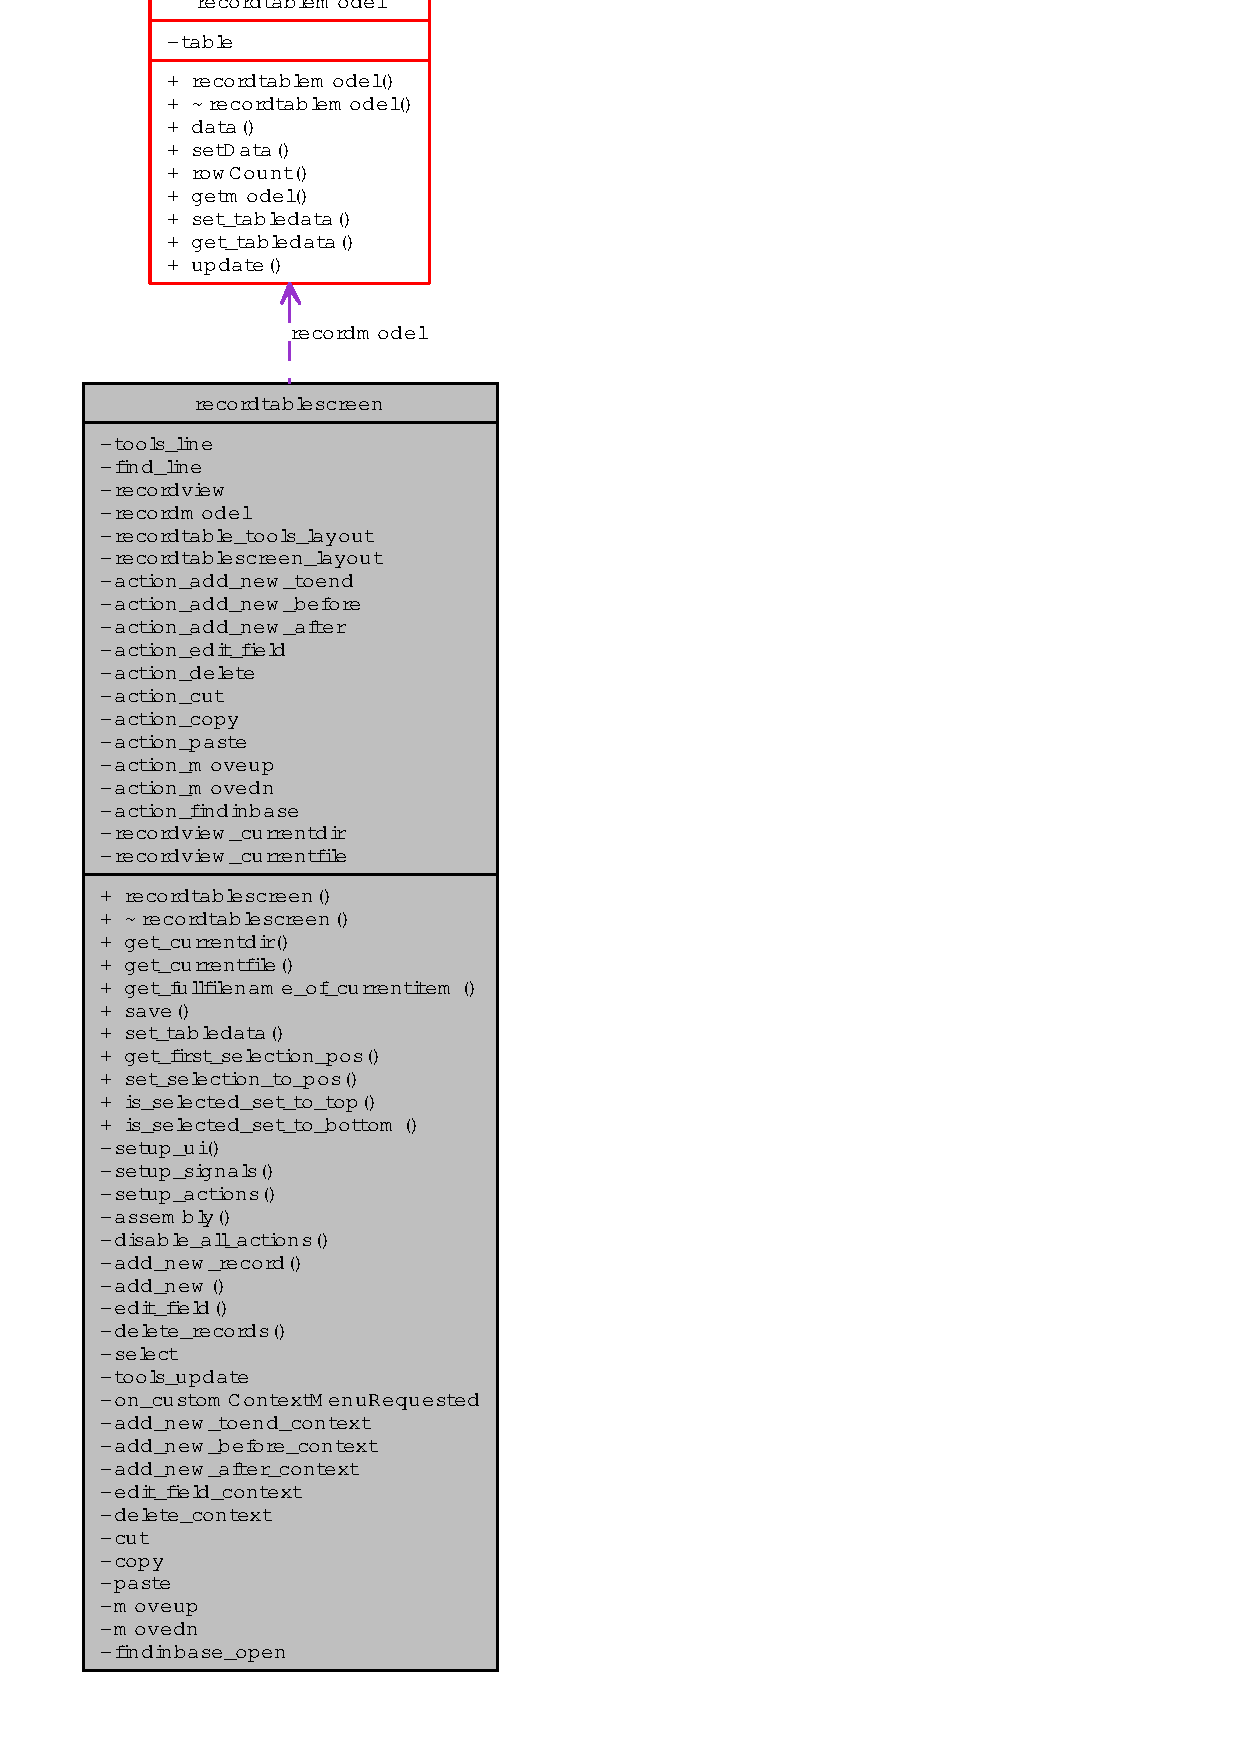
\includegraphics[width=121pt]{classrecordtablescreen__coll__graph}
\end{center}
\end{figure}
\subsection*{Public Member Functions}
\begin{CompactItemize}
\item 
{\bf recordtablescreen} (QWidget $\ast$parent=0)
\item 
virtual {\bf $\sim$recordtablescreen} ()
\item 
QString {\bf get\_\-currentdir} (void)
\item 
QString {\bf get\_\-currentfile} (void)
\item 
QString {\bf get\_\-fullfilename\_\-of\_\-currentitem} (void)
\item 
void {\bf save} (void)
\item 
void {\bf set\_\-tabledata} ({\bf recordtabledata} $\ast$)
\item 
int {\bf get\_\-first\_\-selection\_\-pos} (void)
\item 
void {\bf set\_\-selection\_\-to\_\-pos} (int pos)
\item 
bool {\bf is\_\-selected\_\-set\_\-to\_\-top} (void)
\item 
bool {\bf is\_\-selected\_\-set\_\-to\_\-bottom} (void)
\end{CompactItemize}
\subsection*{Private Slots}
\begin{CompactItemize}
\item 
void {\bf select} (const QModel\-Index \&index)
\item 
void {\bf tools\_\-update} (void)
\item 
void {\bf on\_\-custom\-Context\-Menu\-Requested} (const QPoint \&pos)
\item 
void {\bf add\_\-new\_\-toend\_\-context} (void)
\item 
void {\bf add\_\-new\_\-before\_\-context} (void)
\item 
void {\bf add\_\-new\_\-after\_\-context} (void)
\item 
void {\bf edit\_\-field\_\-context} (void)
\item 
void {\bf delete\_\-context} (void)
\item 
void {\bf cut} (void)
\item 
void {\bf copy} (void)
\item 
void {\bf paste} (void)
\item 
void {\bf moveup} (void)
\item 
void {\bf movedn} (void)
\item 
void {\bf findinbase\_\-open} (void)
\end{CompactItemize}
\subsection*{Private Member Functions}
\begin{CompactItemize}
\item 
void {\bf setup\_\-ui} (void)
\item 
void {\bf setup\_\-signals} (void)
\item 
void {\bf setup\_\-actions} (void)
\item 
void {\bf assembly} (void)
\item 
void {\bf disable\_\-all\_\-actions} (void)
\item 
void {\bf add\_\-new\_\-record} (int mode)
\item 
void {\bf add\_\-new} (int mode, QString name, QString author, QString url, QString tags, QString text)
\item 
void {\bf edit\_\-field} (int pos, QString name, QString author, QString url, QString tags)
\item 
void {\bf delete\_\-records} (void)
\end{CompactItemize}
\subsection*{Private Attributes}
\begin{CompactItemize}
\item 
QTool\-Bar $\ast$ {\bf tools\_\-line}
\item 
QTool\-Bar $\ast$ {\bf find\_\-line}
\item 
QList\-View $\ast$ {\bf recordview}
\item 
{\bf recordtablemodel} $\ast$ {\bf recordmodel}
\item 
QHBox\-Layout $\ast$ {\bf recordtable\_\-tools\_\-layout}
\item 
QVBox\-Layout $\ast$ {\bf recordtablescreen\_\-layout}
\item 
QAction $\ast$ {\bf action\_\-add\_\-new\_\-toend}
\item 
QAction $\ast$ {\bf action\_\-add\_\-new\_\-before}
\item 
QAction $\ast$ {\bf action\_\-add\_\-new\_\-after}
\item 
QAction $\ast$ {\bf action\_\-edit\_\-field}
\item 
QAction $\ast$ {\bf action\_\-delete}
\item 
QAction $\ast$ {\bf action\_\-cut}
\item 
QAction $\ast$ {\bf action\_\-copy}
\item 
QAction $\ast$ {\bf action\_\-paste}
\item 
QAction $\ast$ {\bf action\_\-moveup}
\item 
QAction $\ast$ {\bf action\_\-movedn}
\item 
QAction $\ast$ {\bf action\_\-findinbase}
\item 
QString {\bf recordview\_\-currentdir}
\item 
QString {\bf recordview\_\-currentfile}
\end{CompactItemize}


\subsection{Detailed Description}




Definition at line 15 of file recordtablescreen.h.

\subsection{Constructor \& Destructor Documentation}
\index{recordtablescreen@{recordtablescreen}!recordtablescreen@{recordtablescreen}}
\index{recordtablescreen@{recordtablescreen}!recordtablescreen@{recordtablescreen}}
\subsubsection{\setlength{\rightskip}{0pt plus 5cm}recordtablescreen::recordtablescreen (QWidget $\ast$ {\em parent} = {\tt 0})}\label{classrecordtablescreen_2542f57dfdd42389520d5f7d6963493f}




Definition at line 14 of file recordtablescreen.cpp.

References assembly(), recordmodel, recordview, recordview\_\-currentdir, recordview\_\-currentfile, setup\_\-actions(), setup\_\-signals(), and setup\_\-ui().

Here is the call graph for this function:\begin{figure}[H]
\begin{center}
\leavevmode
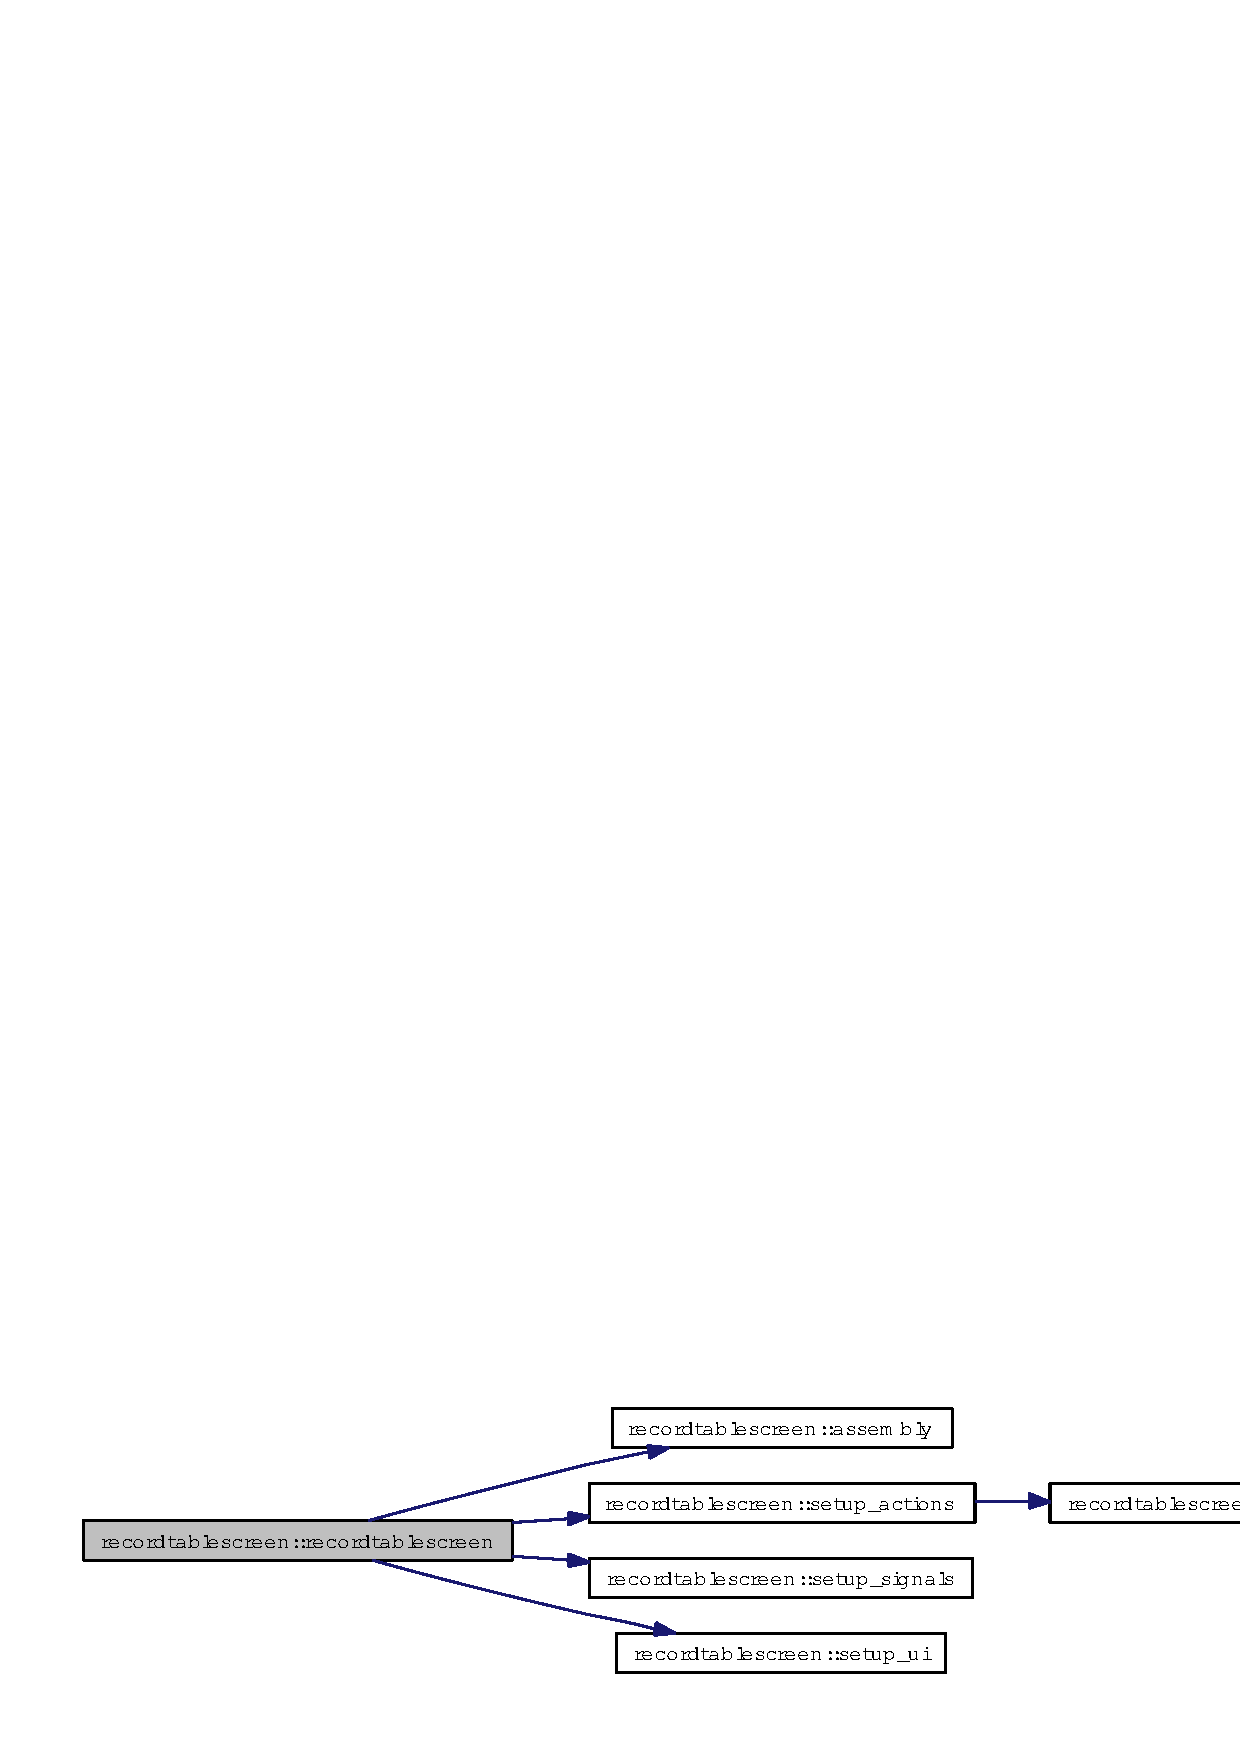
\includegraphics[width=359pt]{classrecordtablescreen_2542f57dfdd42389520d5f7d6963493f_cgraph}
\end{center}
\end{figure}
\index{recordtablescreen@{recordtablescreen}!~recordtablescreen@{$\sim$recordtablescreen}}
\index{~recordtablescreen@{$\sim$recordtablescreen}!recordtablescreen@{recordtablescreen}}
\subsubsection{\setlength{\rightskip}{0pt plus 5cm}recordtablescreen::$\sim$recordtablescreen ()\hspace{0.3cm}{\tt  [virtual]}}\label{classrecordtablescreen_832d2a50320b57218eaa071b4692eb7f}




Definition at line 37 of file recordtablescreen.cpp.

\subsection{Member Function Documentation}
\index{recordtablescreen@{recordtablescreen}!get_currentdir@{get\_\-currentdir}}
\index{get_currentdir@{get\_\-currentdir}!recordtablescreen@{recordtablescreen}}
\subsubsection{\setlength{\rightskip}{0pt plus 5cm}QString recordtablescreen::get\_\-currentdir (void)}\label{classrecordtablescreen_5f419b091a8911fa8be695b6c5956e7e}




Definition at line 233 of file recordtablescreen.cpp.

References recordview\_\-currentdir.

Referenced by mainwindow::save\_\-current\_\-record\_\-text().

Here is the caller graph for this function:\begin{figure}[H]
\begin{center}
\leavevmode
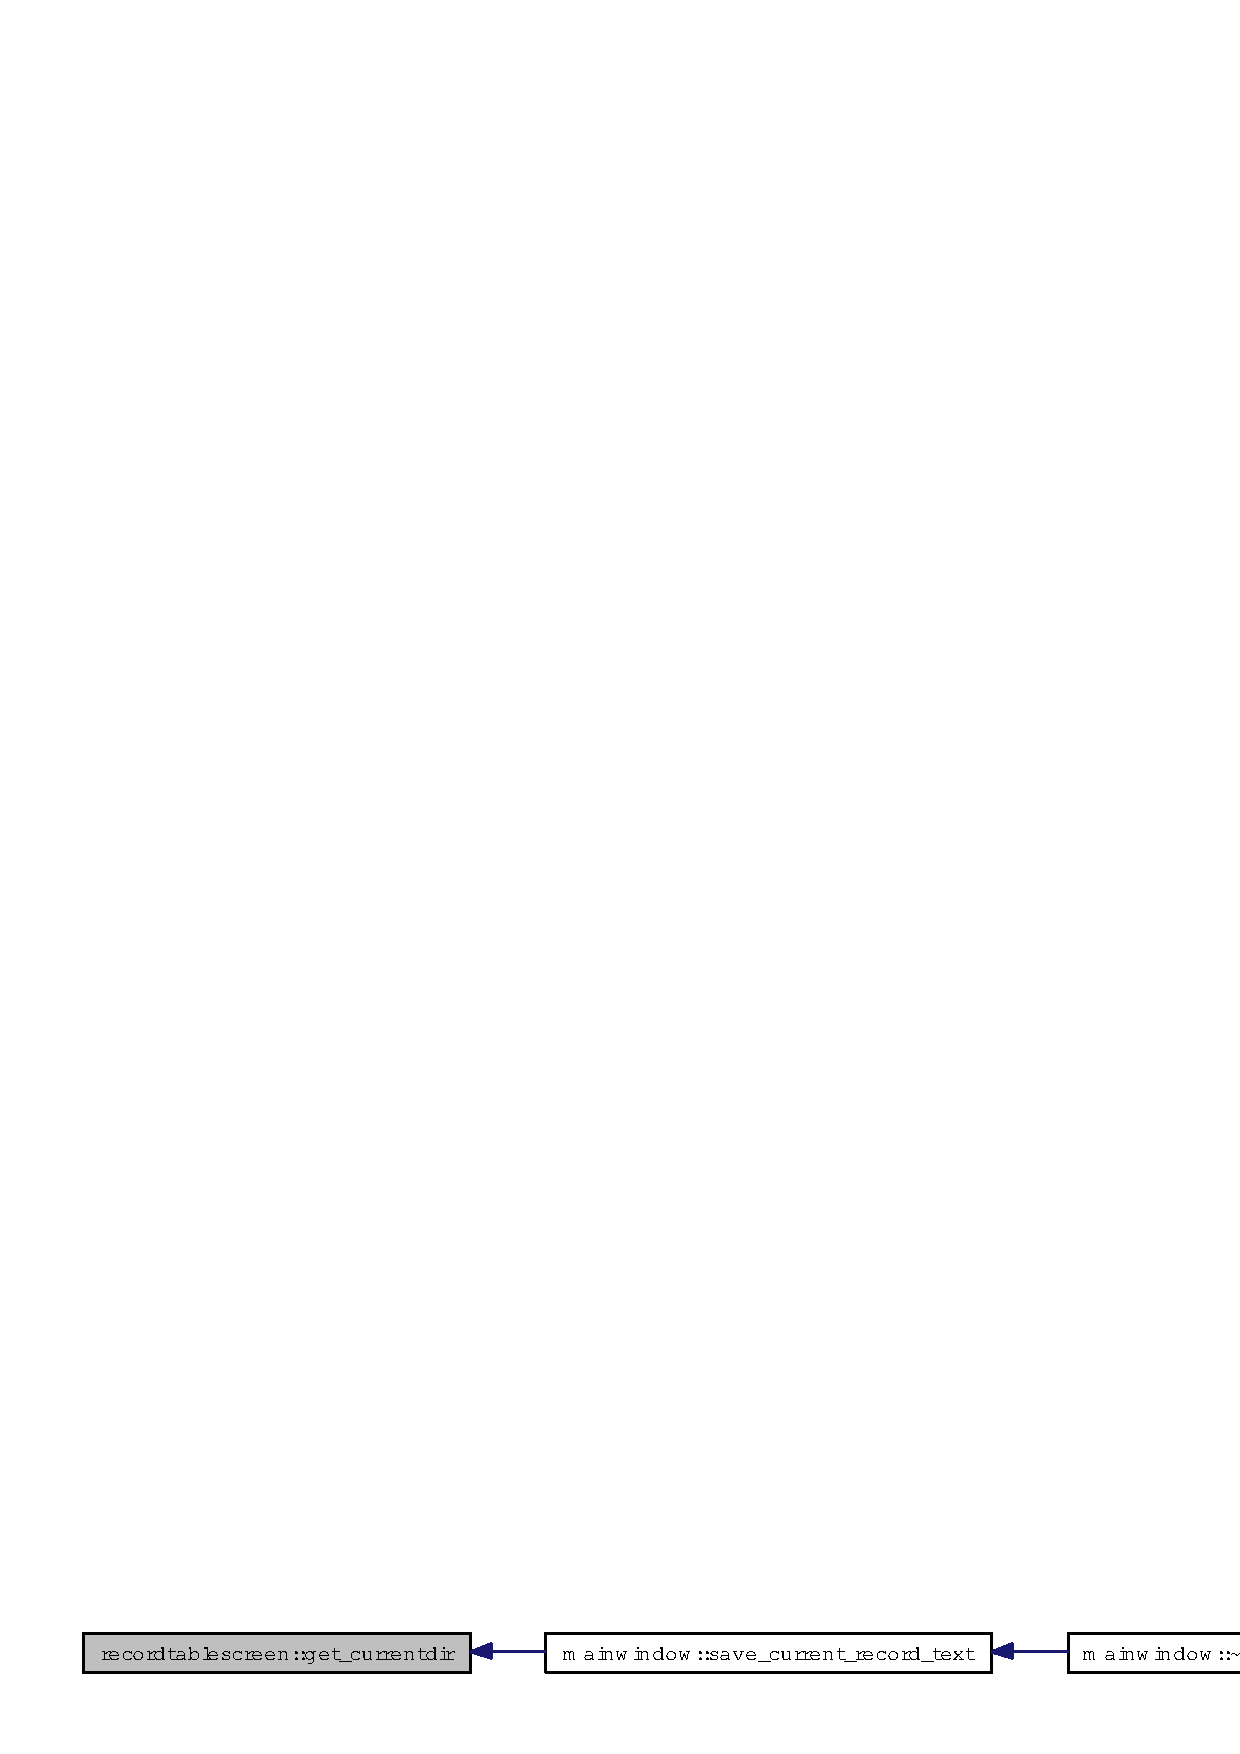
\includegraphics[width=338pt]{classrecordtablescreen_5f419b091a8911fa8be695b6c5956e7e_icgraph}
\end{center}
\end{figure}
\index{recordtablescreen@{recordtablescreen}!get_currentfile@{get\_\-currentfile}}
\index{get_currentfile@{get\_\-currentfile}!recordtablescreen@{recordtablescreen}}
\subsubsection{\setlength{\rightskip}{0pt plus 5cm}QString recordtablescreen::get\_\-currentfile (void)}\label{classrecordtablescreen_e7502491e7959dc271a55ed39d255a9d}




Definition at line 239 of file recordtablescreen.cpp.

References recordview\_\-currentfile.

Referenced by mainwindow::save\_\-current\_\-record\_\-text().

Here is the caller graph for this function:\begin{figure}[H]
\begin{center}
\leavevmode
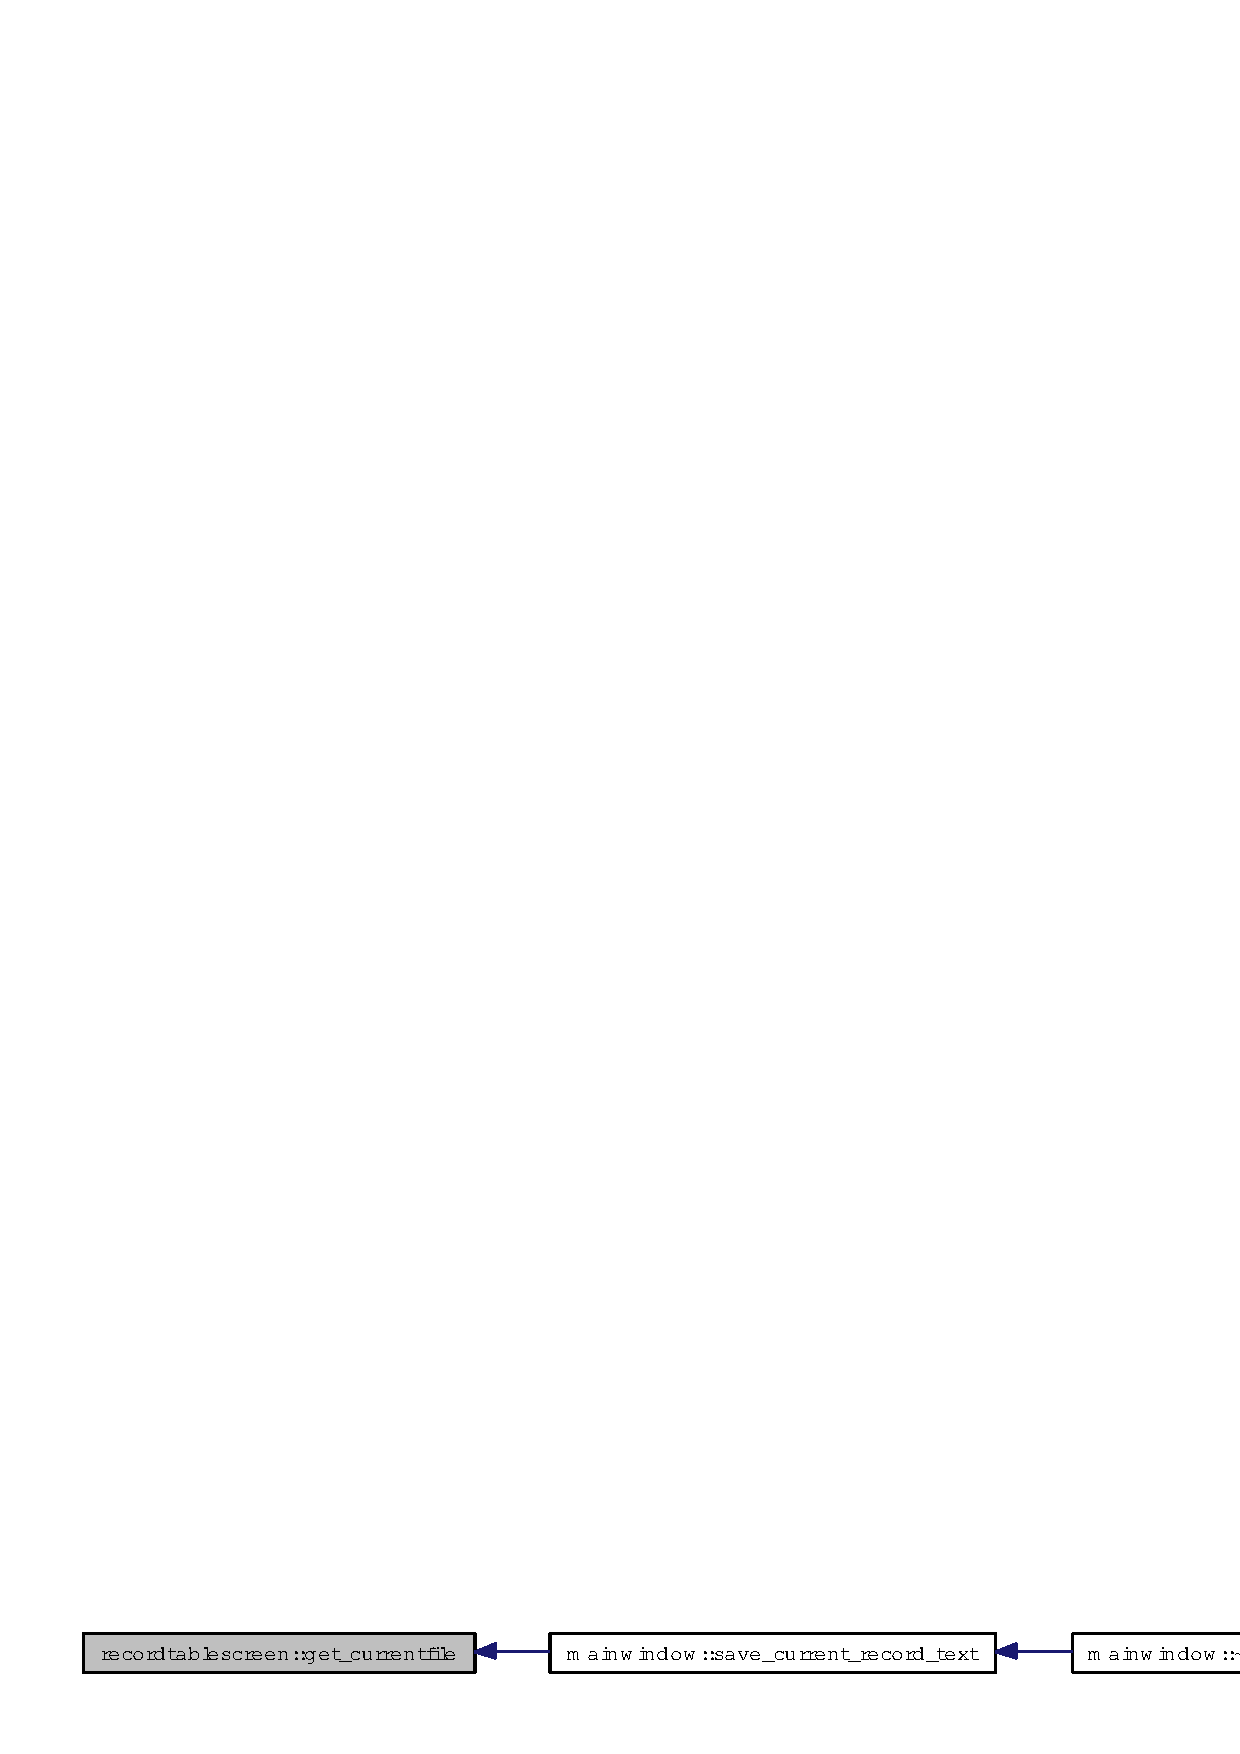
\includegraphics[width=339pt]{classrecordtablescreen_e7502491e7959dc271a55ed39d255a9d_icgraph}
\end{center}
\end{figure}
\index{recordtablescreen@{recordtablescreen}!get_fullfilename_of_currentitem@{get\_\-fullfilename\_\-of\_\-currentitem}}
\index{get_fullfilename_of_currentitem@{get\_\-fullfilename\_\-of\_\-currentitem}!recordtablescreen@{recordtablescreen}}
\subsubsection{\setlength{\rightskip}{0pt plus 5cm}QString recordtablescreen::get\_\-fullfilename\_\-of\_\-currentitem (void)}\label{classrecordtablescreen_a3fac56820514280445d9ef0de9f1632}




Definition at line 246 of file recordtablescreen.cpp.

References appconfig::get\_\-tetradir(), mytetraconfig, recordview\_\-currentdir, and recordview\_\-currentfile.

Referenced by mainwindow::save\_\-current\_\-record\_\-text().

Here is the call graph for this function:\begin{figure}[H]
\begin{center}
\leavevmode
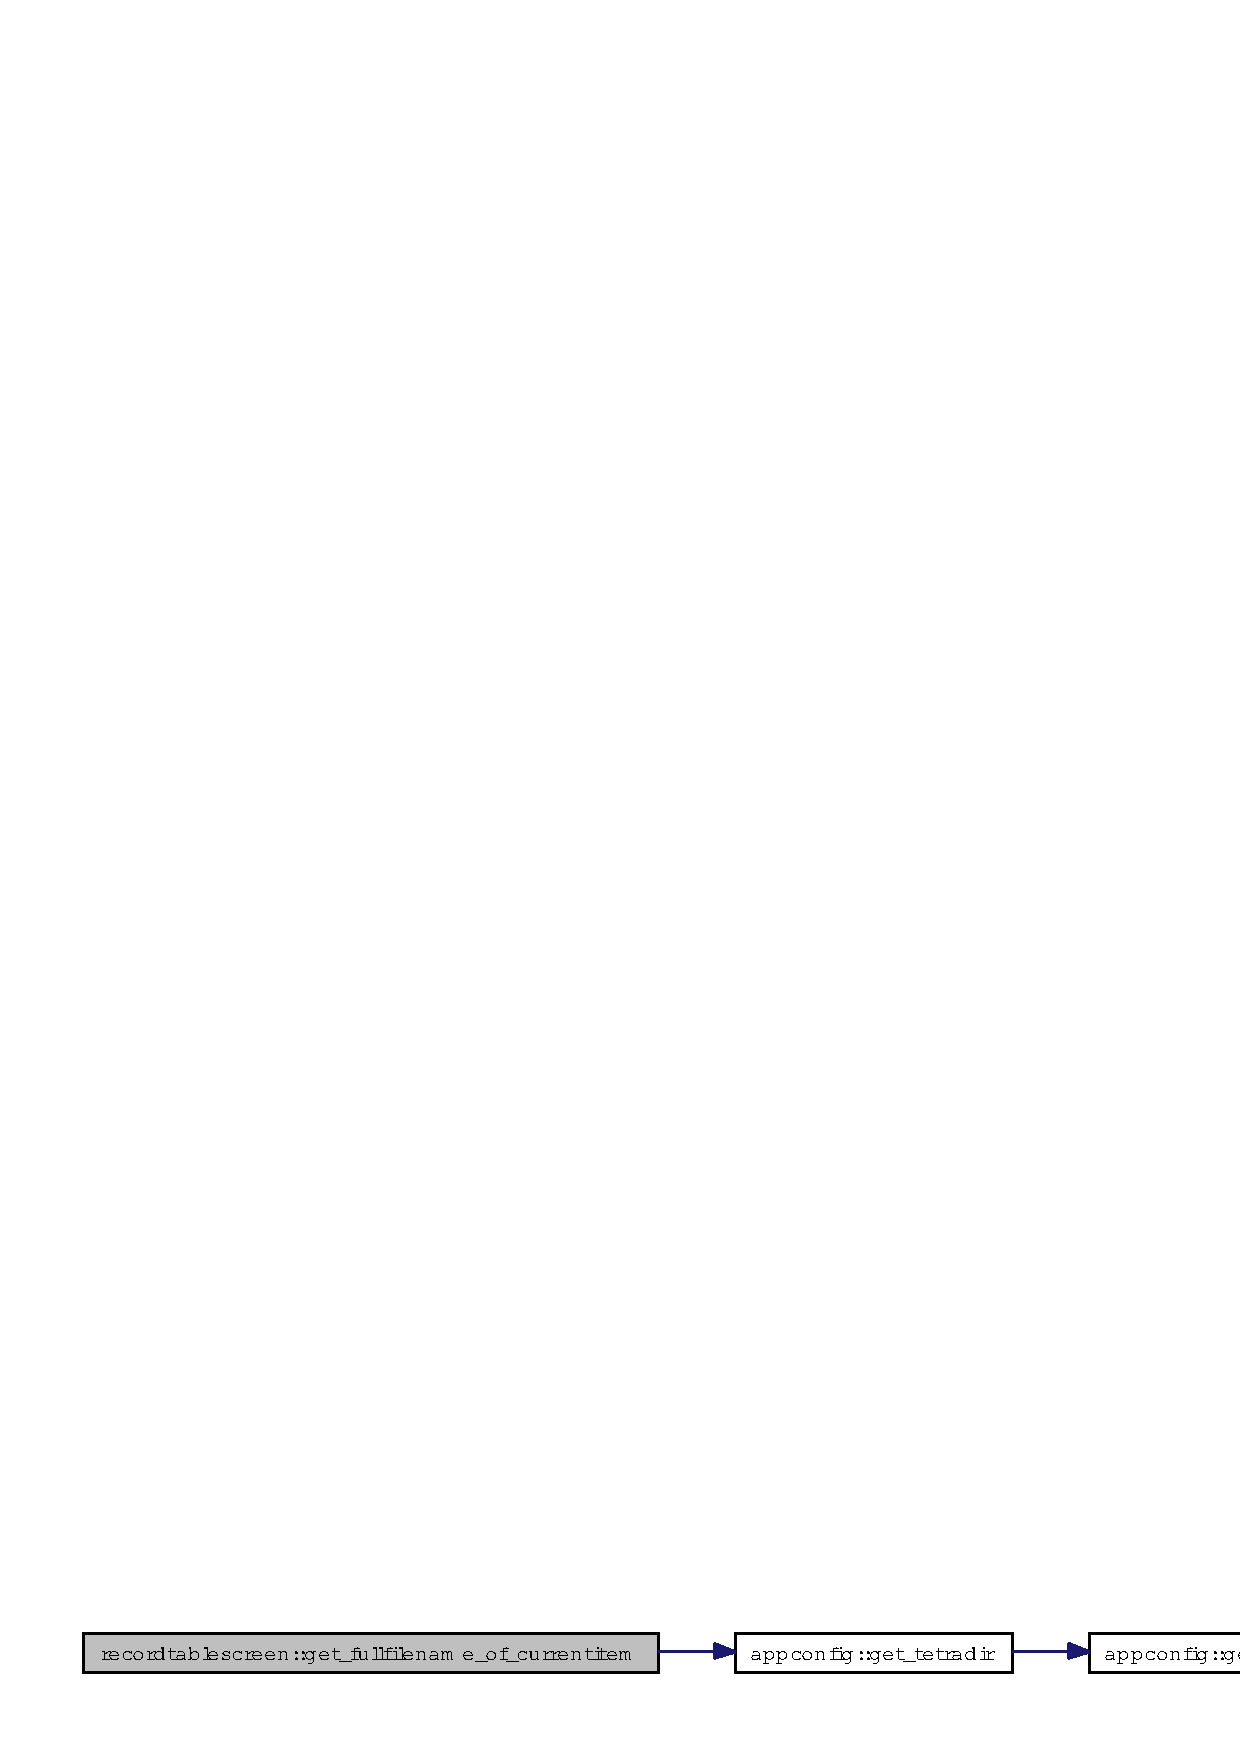
\includegraphics[width=396pt]{classrecordtablescreen_a3fac56820514280445d9ef0de9f1632_cgraph}
\end{center}
\end{figure}


Here is the caller graph for this function:\begin{figure}[H]
\begin{center}
\leavevmode
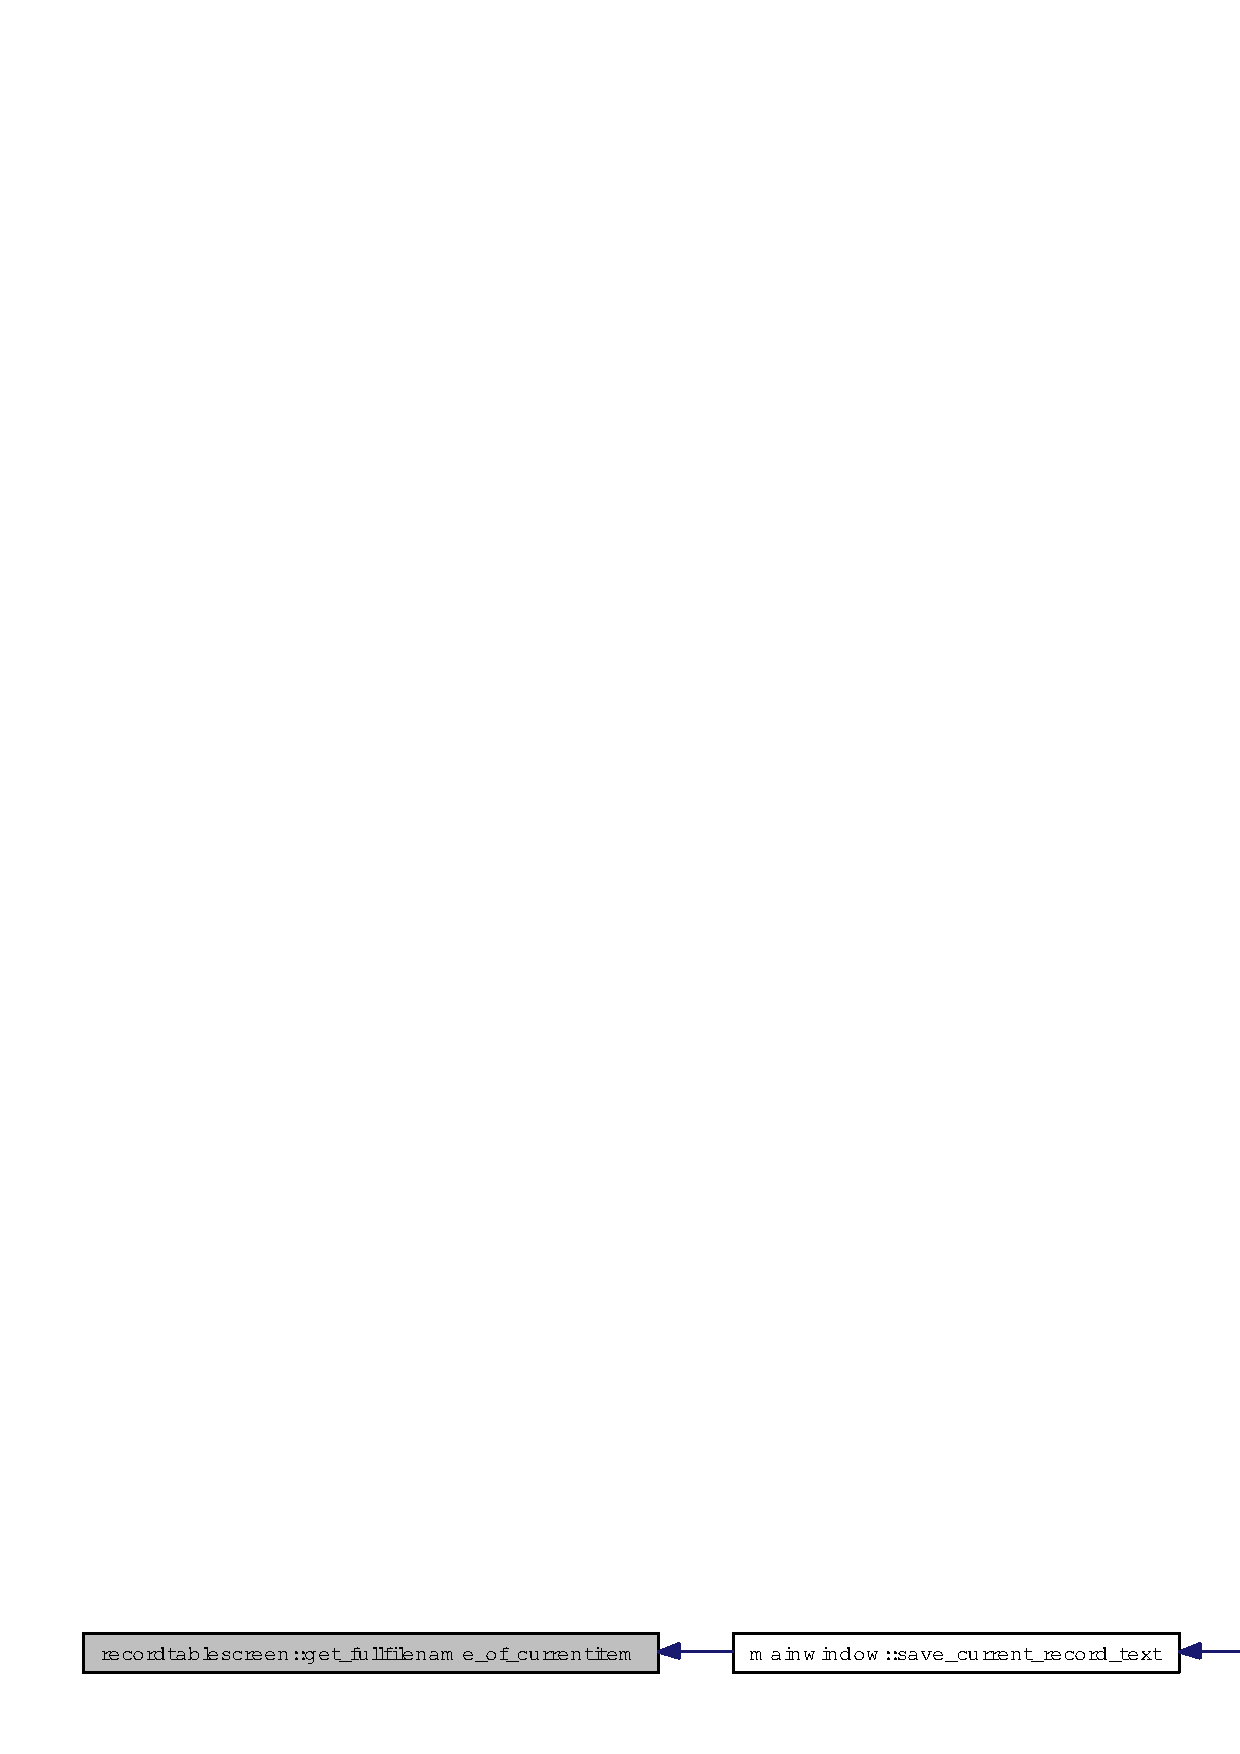
\includegraphics[width=383pt]{classrecordtablescreen_a3fac56820514280445d9ef0de9f1632_icgraph}
\end{center}
\end{figure}
\index{recordtablescreen@{recordtablescreen}!save@{save}}
\index{save@{save}!recordtablescreen@{recordtablescreen}}
\subsubsection{\setlength{\rightskip}{0pt plus 5cm}void recordtablescreen::save (void)}\label{classrecordtablescreen_8586c6a01418e5ef3f3561f421f4beea}


\index{recordtablescreen@{recordtablescreen}!set_tabledata@{set\_\-tabledata}}
\index{set_tabledata@{set\_\-tabledata}!recordtablescreen@{recordtablescreen}}
\subsubsection{\setlength{\rightskip}{0pt plus 5cm}void recordtablescreen::set\_\-tabledata ({\bf recordtabledata} $\ast$)}\label{classrecordtablescreen_e1572a908c5e8c72af3ed0000375e2dd}




Definition at line 197 of file recordtablescreen.cpp.

References recordmodel, recordview, recordview\_\-currentdir, recordview\_\-currentfile, recordtablemodel::row\-Count(), and recordtablemodel::set\_\-tabledata().

Here is the call graph for this function:\begin{figure}[H]
\begin{center}
\leavevmode
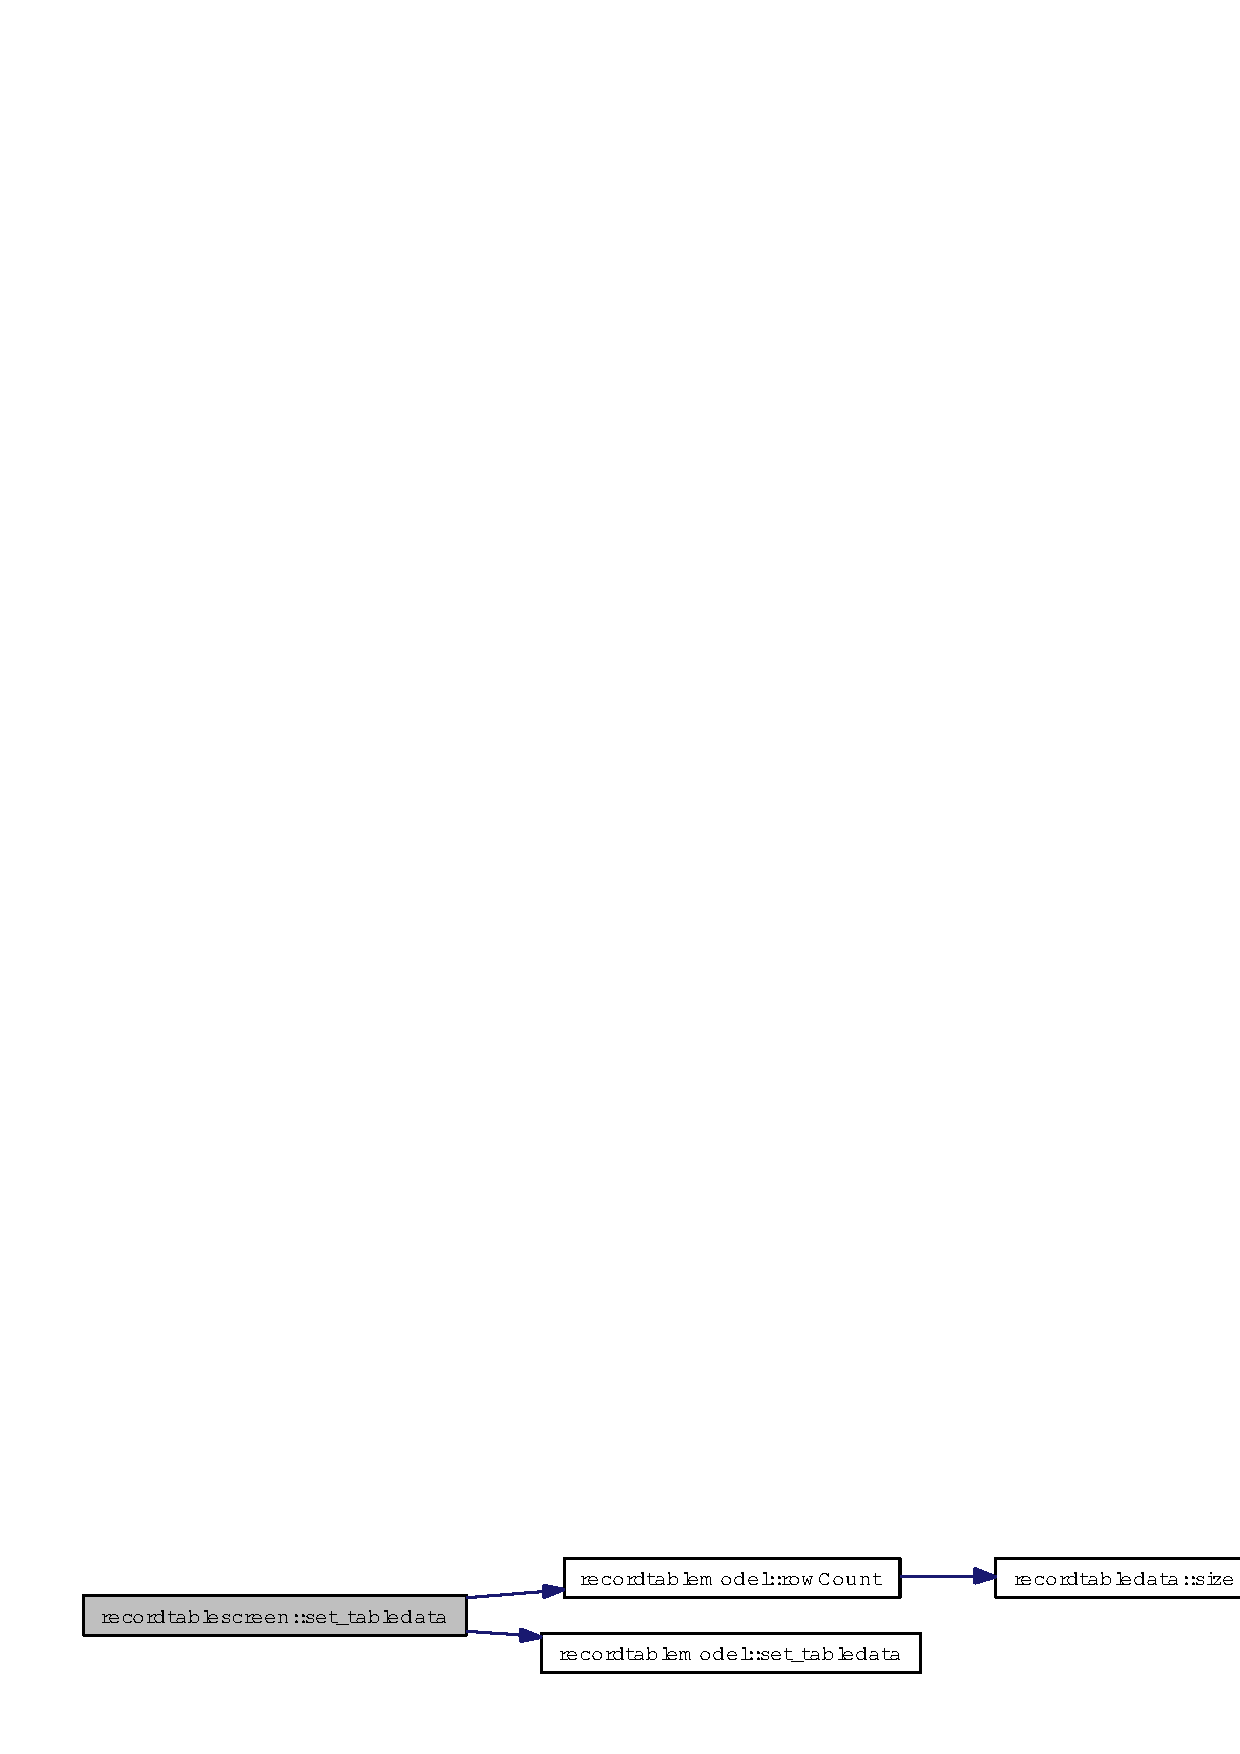
\includegraphics[width=303pt]{classrecordtablescreen_e1572a908c5e8c72af3ed0000375e2dd_cgraph}
\end{center}
\end{figure}
\index{recordtablescreen@{recordtablescreen}!get_first_selection_pos@{get\_\-first\_\-selection\_\-pos}}
\index{get_first_selection_pos@{get\_\-first\_\-selection\_\-pos}!recordtablescreen@{recordtablescreen}}
\subsubsection{\setlength{\rightskip}{0pt plus 5cm}int recordtablescreen::get\_\-first\_\-selection\_\-pos (void)}\label{classrecordtablescreen_edf8ac561d0f33acf6af0fe63fbc8a91}




Definition at line 817 of file recordtablescreen.cpp.

References recordview.

Referenced by add\_\-new(), is\_\-selected\_\-set\_\-to\_\-bottom(), is\_\-selected\_\-set\_\-to\_\-top(), movedn(), moveup(), and mainwindow::save\_\-recordtable\_\-position().

Here is the caller graph for this function:\begin{figure}[H]
\begin{center}
\leavevmode
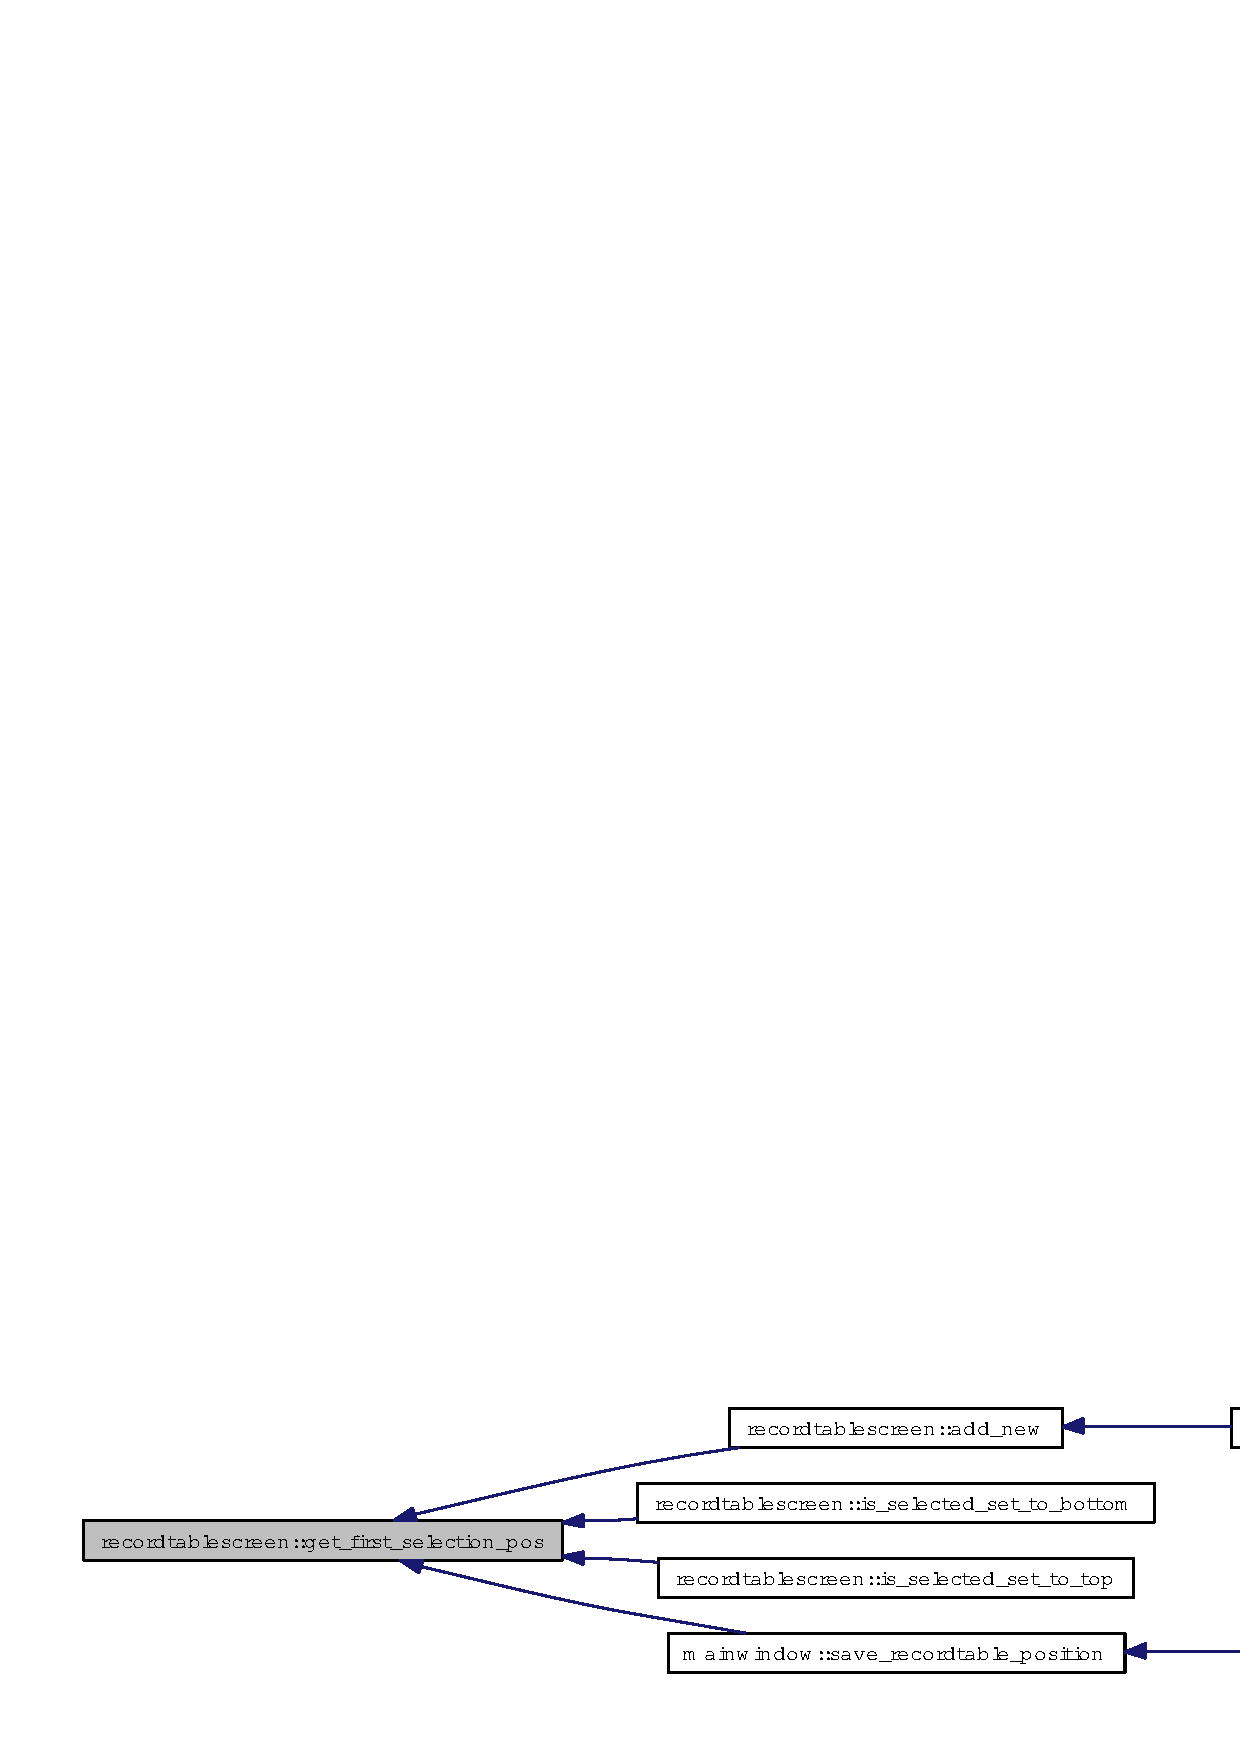
\includegraphics[width=396pt]{classrecordtablescreen_edf8ac561d0f33acf6af0fe63fbc8a91_icgraph}
\end{center}
\end{figure}
\index{recordtablescreen@{recordtablescreen}!set_selection_to_pos@{set\_\-selection\_\-to\_\-pos}}
\index{set_selection_to_pos@{set\_\-selection\_\-to\_\-pos}!recordtablescreen@{recordtablescreen}}
\subsubsection{\setlength{\rightskip}{0pt plus 5cm}void recordtablescreen::set\_\-selection\_\-to\_\-pos (int {\em pos})}\label{classrecordtablescreen_3694df3f0aae7c3b1ea3913e81b94f90}




Definition at line 844 of file recordtablescreen.cpp.

References recordmodel, and recordview.

Referenced by movedn(), moveup(), and mainwindow::set\_\-recordtable\_\-position().

Here is the caller graph for this function:\begin{figure}[H]
\begin{center}
\leavevmode
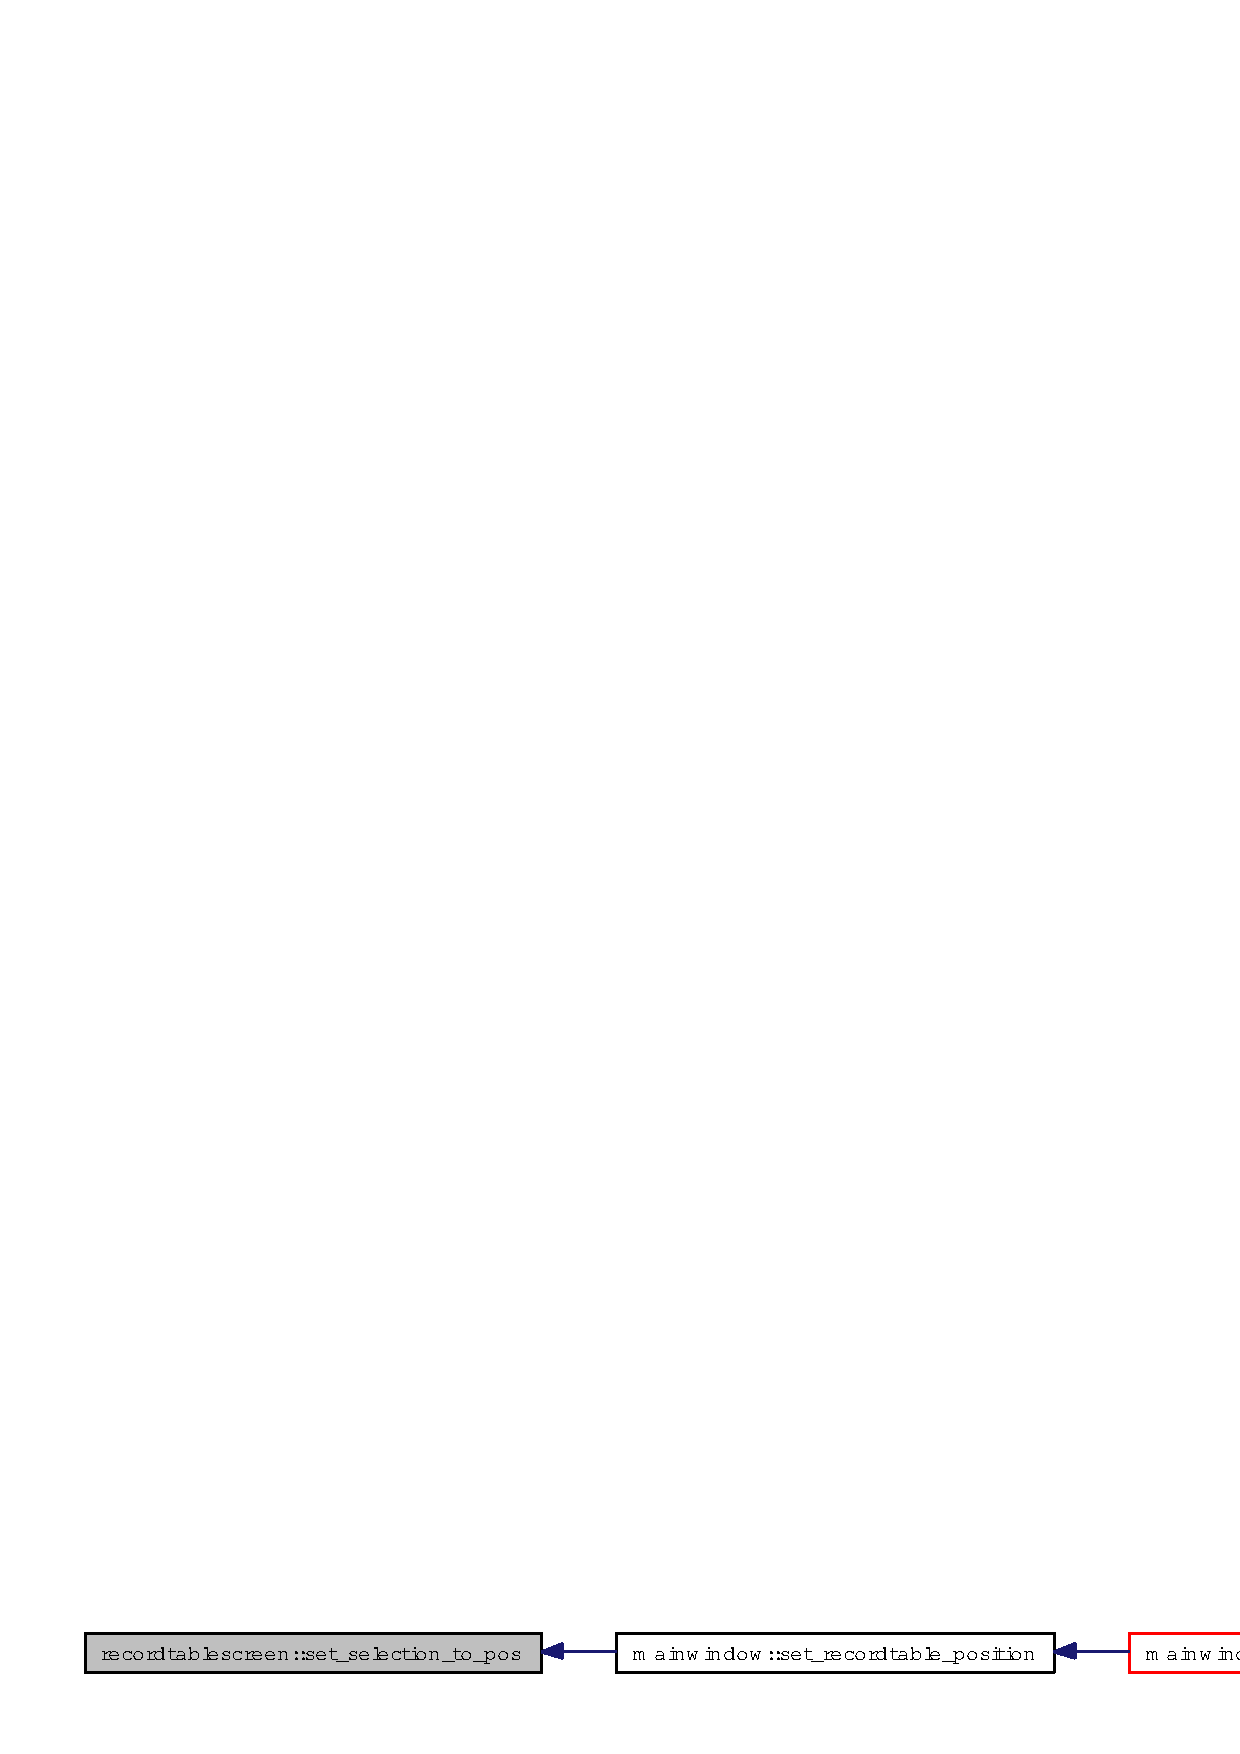
\includegraphics[width=388pt]{classrecordtablescreen_3694df3f0aae7c3b1ea3913e81b94f90_icgraph}
\end{center}
\end{figure}
\index{recordtablescreen@{recordtablescreen}!is_selected_set_to_top@{is\_\-selected\_\-set\_\-to\_\-top}}
\index{is_selected_set_to_top@{is\_\-selected\_\-set\_\-to\_\-top}!recordtablescreen@{recordtablescreen}}
\subsubsection{\setlength{\rightskip}{0pt plus 5cm}bool recordtablescreen::is\_\-selected\_\-set\_\-to\_\-top (void)}\label{classrecordtablescreen_c84c840f480e4e03017e4f3056388d3d}




Definition at line 829 of file recordtablescreen.cpp.

References get\_\-first\_\-selection\_\-pos().

Referenced by tools\_\-update().

Here is the call graph for this function:\begin{figure}[H]
\begin{center}
\leavevmode
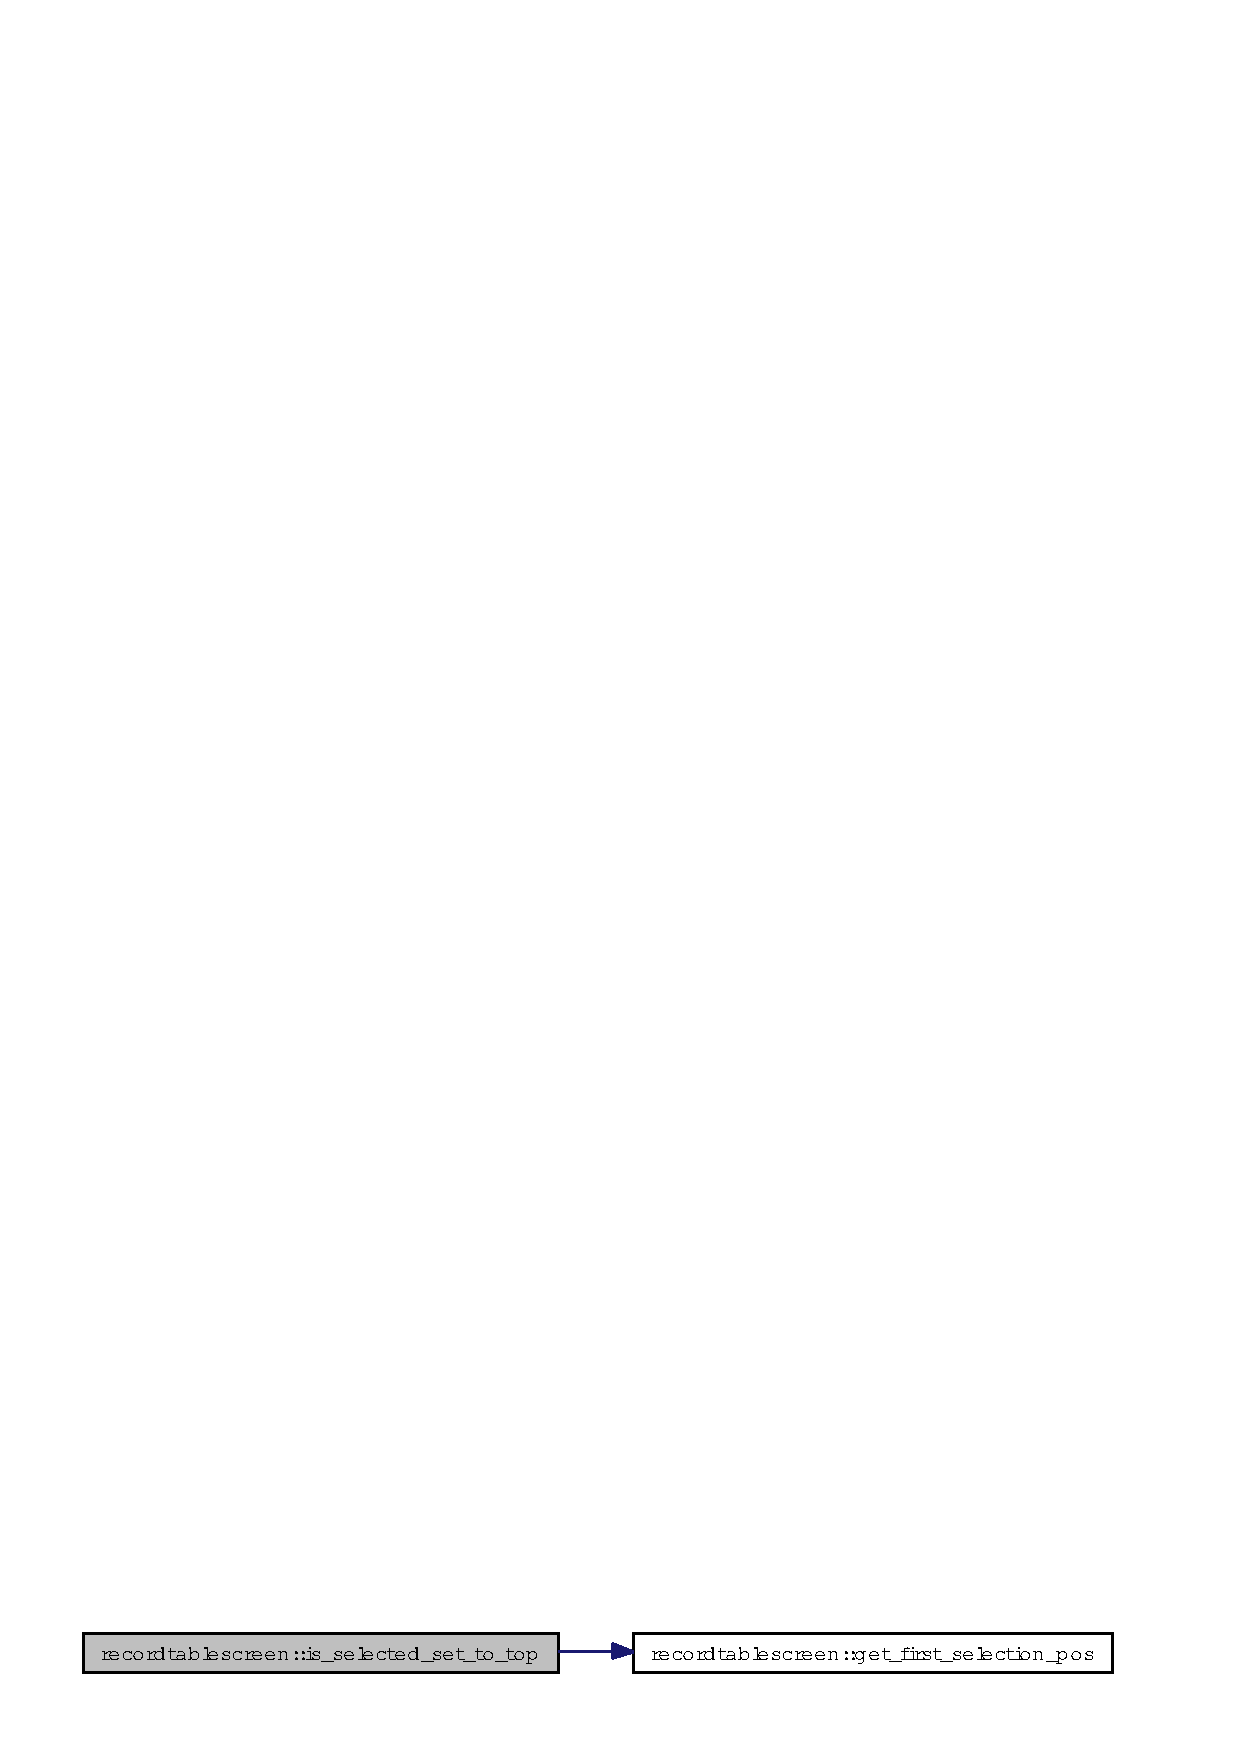
\includegraphics[width=269pt]{classrecordtablescreen_c84c840f480e4e03017e4f3056388d3d_cgraph}
\end{center}
\end{figure}
\index{recordtablescreen@{recordtablescreen}!is_selected_set_to_bottom@{is\_\-selected\_\-set\_\-to\_\-bottom}}
\index{is_selected_set_to_bottom@{is\_\-selected\_\-set\_\-to\_\-bottom}!recordtablescreen@{recordtablescreen}}
\subsubsection{\setlength{\rightskip}{0pt plus 5cm}bool recordtablescreen::is\_\-selected\_\-set\_\-to\_\-bottom (void)}\label{classrecordtablescreen_c73f9f801e76c4cb83556dd1b99d8192}




Definition at line 836 of file recordtablescreen.cpp.

References get\_\-first\_\-selection\_\-pos(), and recordview.

Referenced by tools\_\-update().

Here is the call graph for this function:\begin{figure}[H]
\begin{center}
\leavevmode
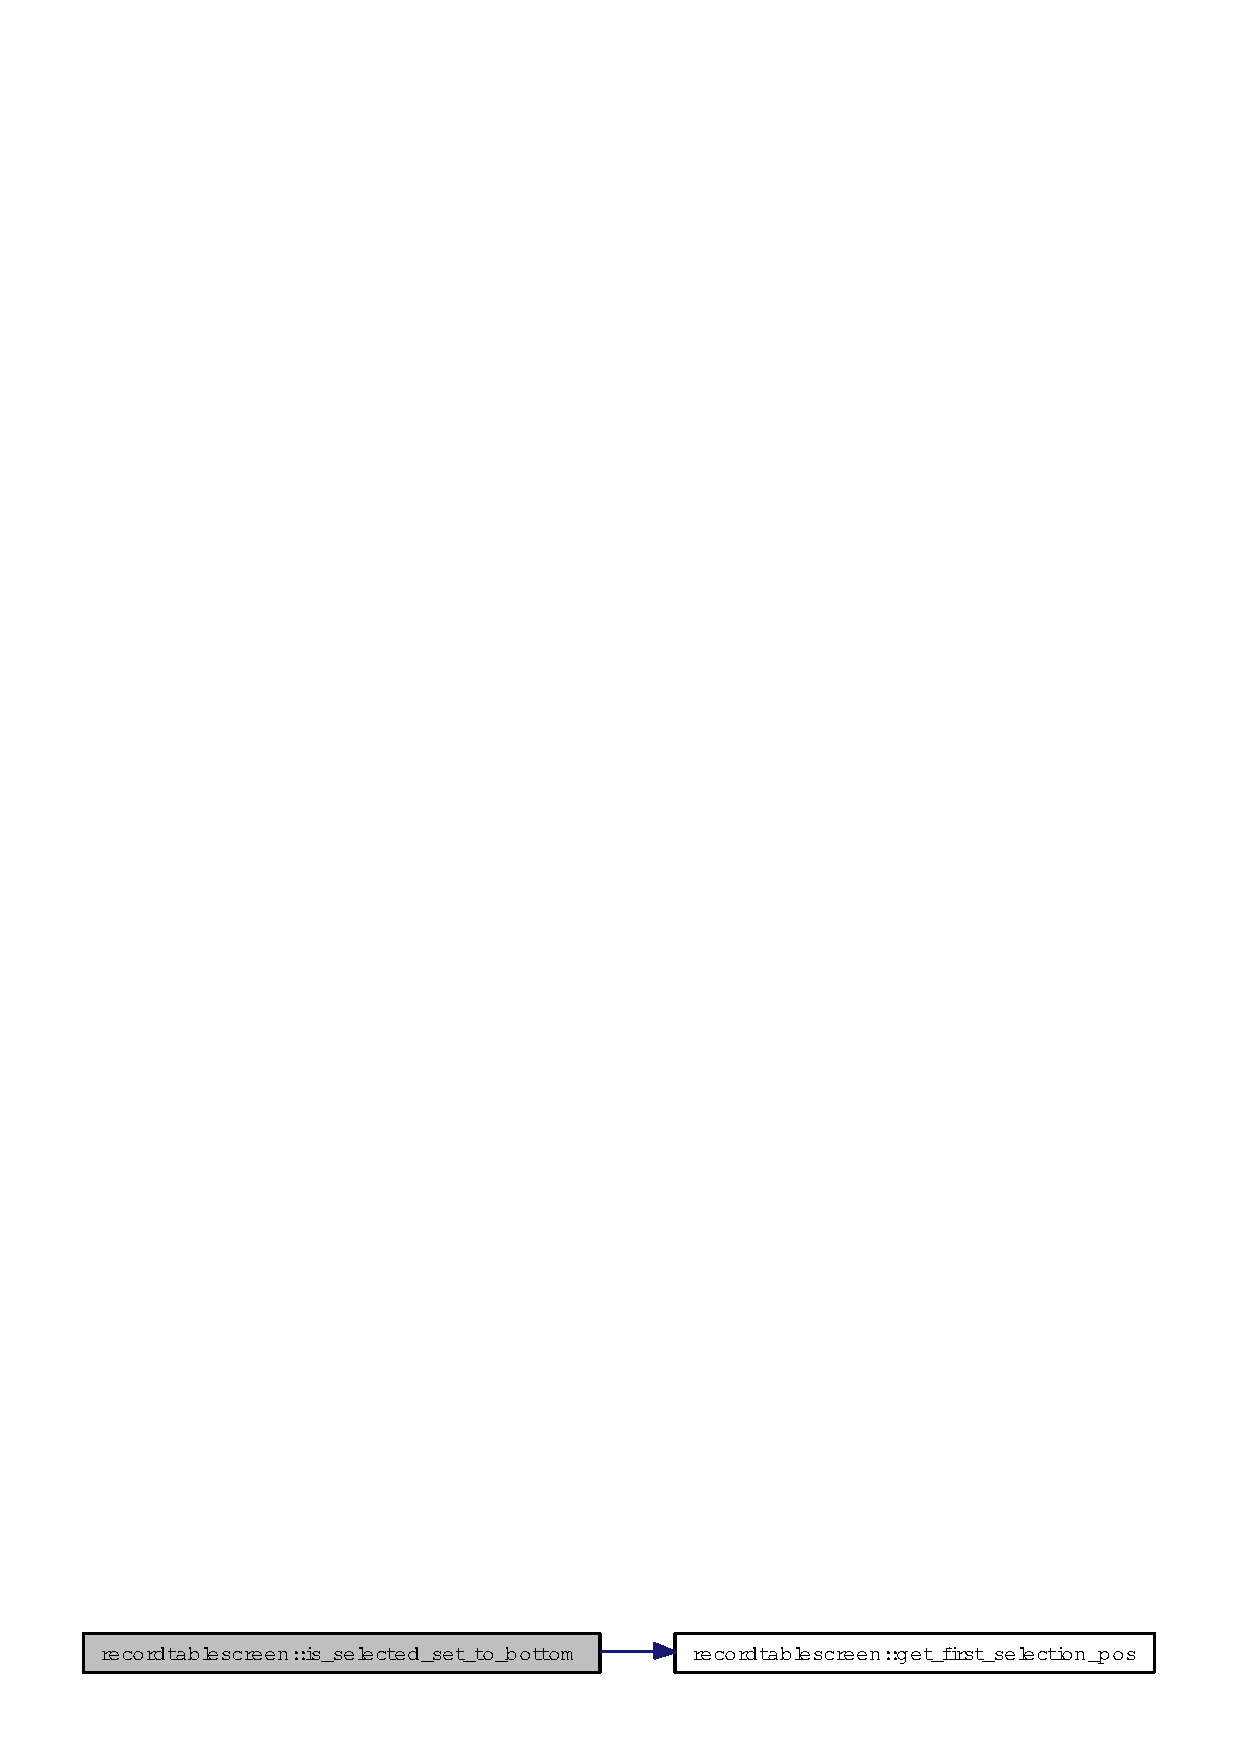
\includegraphics[width=279pt]{classrecordtablescreen_c73f9f801e76c4cb83556dd1b99d8192_cgraph}
\end{center}
\end{figure}
\index{recordtablescreen@{recordtablescreen}!select@{select}}
\index{select@{select}!recordtablescreen@{recordtablescreen}}
\subsubsection{\setlength{\rightskip}{0pt plus 5cm}void recordtablescreen::select (const QModel\-Index \& {\em index})\hspace{0.3cm}{\tt  [private, slot]}}\label{classrecordtablescreen_55bc3b168d846297e2107ea29ee24f7a}




Definition at line 254 of file recordtablescreen.cpp.

References critical\_\-error(), recordtabledata::get\_\-field(), recordtablemodel::get\_\-tabledata(), appconfig::get\_\-tetradir(), mytetraconfig, recordmodel, recordview\_\-currentdir, recordview\_\-currentfile, metaeditor::set\_\-author(), metaeditor::set\_\-name(), metaeditor::set\_\-tags(), editor::set\_\-textarea(), and metaeditor::set\_\-url().

Referenced by edit\_\-field\_\-context(), and setup\_\-signals().\index{recordtablescreen@{recordtablescreen}!tools_update@{tools\_\-update}}
\index{tools_update@{tools\_\-update}!recordtablescreen@{recordtablescreen}}
\subsubsection{\setlength{\rightskip}{0pt plus 5cm}void recordtablescreen::tools\_\-update (void)\hspace{0.3cm}{\tt  [private, slot]}}\label{classrecordtablescreen_a4b0a512d0caf52495f5cb2883fcb2f8}




Definition at line 657 of file recordtablescreen.cpp.

References action\_\-add\_\-new\_\-after, action\_\-add\_\-new\_\-before, action\_\-add\_\-new\_\-toend, action\_\-copy, action\_\-cut, action\_\-delete, action\_\-edit\_\-field, action\_\-movedn, action\_\-moveup, action\_\-paste, disable\_\-all\_\-actions(), is\_\-selected\_\-set\_\-to\_\-bottom(), is\_\-selected\_\-set\_\-to\_\-top(), and recordview.

Referenced by setup\_\-signals().\index{recordtablescreen@{recordtablescreen}!on_customContextMenuRequested@{on\_\-customContextMenuRequested}}
\index{on_customContextMenuRequested@{on\_\-customContextMenuRequested}!recordtablescreen@{recordtablescreen}}
\subsubsection{\setlength{\rightskip}{0pt plus 5cm}void recordtablescreen::on\_\-custom\-Context\-Menu\-Requested (const QPoint \& {\em pos})\hspace{0.3cm}{\tt  [private, slot]}}\label{classrecordtablescreen_4d456453a98a1cda55cf374d4178f6a8}




Definition at line 747 of file recordtablescreen.cpp.

References action\_\-add\_\-new\_\-after, action\_\-add\_\-new\_\-before, action\_\-add\_\-new\_\-toend, action\_\-copy, action\_\-cut, action\_\-delete, action\_\-edit\_\-field, action\_\-paste, and recordview.

Referenced by setup\_\-signals().\index{recordtablescreen@{recordtablescreen}!add_new_toend_context@{add\_\-new\_\-toend\_\-context}}
\index{add_new_toend_context@{add\_\-new\_\-toend\_\-context}!recordtablescreen@{recordtablescreen}}
\subsubsection{\setlength{\rightskip}{0pt plus 5cm}void recordtablescreen::add\_\-new\_\-toend\_\-context (void)\hspace{0.3cm}{\tt  [private, slot]}}\label{classrecordtablescreen_15da6524cadb2a7400e53d0c44476d63}




Definition at line 302 of file recordtablescreen.cpp.

References add\_\-new\_\-record(), and ADD\_\-NEW\_\-RECORD\_\-TO\_\-END.

Referenced by setup\_\-actions().\index{recordtablescreen@{recordtablescreen}!add_new_before_context@{add\_\-new\_\-before\_\-context}}
\index{add_new_before_context@{add\_\-new\_\-before\_\-context}!recordtablescreen@{recordtablescreen}}
\subsubsection{\setlength{\rightskip}{0pt plus 5cm}void recordtablescreen::add\_\-new\_\-before\_\-context (void)\hspace{0.3cm}{\tt  [private, slot]}}\label{classrecordtablescreen_ace7ad1829e374ae71e8ca7121fa7607}




Definition at line 311 of file recordtablescreen.cpp.

References add\_\-new\_\-record(), and ADD\_\-NEW\_\-RECORD\_\-BEFORE.

Referenced by setup\_\-actions().\index{recordtablescreen@{recordtablescreen}!add_new_after_context@{add\_\-new\_\-after\_\-context}}
\index{add_new_after_context@{add\_\-new\_\-after\_\-context}!recordtablescreen@{recordtablescreen}}
\subsubsection{\setlength{\rightskip}{0pt plus 5cm}void recordtablescreen::add\_\-new\_\-after\_\-context (void)\hspace{0.3cm}{\tt  [private, slot]}}\label{classrecordtablescreen_22360e9ef1ec9a8ae665250a7cbbfb97}




Definition at line 320 of file recordtablescreen.cpp.

References add\_\-new\_\-record(), and ADD\_\-NEW\_\-RECORD\_\-AFTER.

Referenced by setup\_\-actions().\index{recordtablescreen@{recordtablescreen}!edit_field_context@{edit\_\-field\_\-context}}
\index{edit_field_context@{edit\_\-field\_\-context}!recordtablescreen@{recordtablescreen}}
\subsubsection{\setlength{\rightskip}{0pt plus 5cm}void recordtablescreen::edit\_\-field\_\-context (void)\hspace{0.3cm}{\tt  [private, slot]}}\label{classrecordtablescreen_5dd89302e35d464936f4492e8043204c}




Definition at line 385 of file recordtablescreen.cpp.

References edit\_\-field(), editrecord::get\_\-field(), recordtabledata::get\_\-field(), recordtablemodel::get\_\-tabledata(), recordmodel, recordview, select(), and editrecord::set\_\-field().

Referenced by setup\_\-actions(), and setup\_\-signals().\index{recordtablescreen@{recordtablescreen}!delete_context@{delete\_\-context}}
\index{delete_context@{delete\_\-context}!recordtablescreen@{recordtablescreen}}
\subsubsection{\setlength{\rightskip}{0pt plus 5cm}void recordtablescreen::delete\_\-context (void)\hspace{0.3cm}{\tt  [private, slot]}}\label{classrecordtablescreen_7112dde2ef63a21504b91061c6facd88}




Definition at line 454 of file recordtablescreen.cpp.

References delete\_\-records().

Referenced by setup\_\-actions().\index{recordtablescreen@{recordtablescreen}!cut@{cut}}
\index{cut@{cut}!recordtablescreen@{recordtablescreen}}
\subsubsection{\setlength{\rightskip}{0pt plus 5cm}void recordtablescreen::cut (void)\hspace{0.3cm}{\tt  [private, slot]}}\label{classrecordtablescreen_ff66fb349cc313a39b880a6a24d3a48f}




Definition at line 554 of file recordtablescreen.cpp.

References copy(), and delete\_\-records().

Referenced by setup\_\-actions().\index{recordtablescreen@{recordtablescreen}!copy@{copy}}
\index{copy@{copy}!recordtablescreen@{recordtablescreen}}
\subsubsection{\setlength{\rightskip}{0pt plus 5cm}void recordtablescreen::copy (void)\hspace{0.3cm}{\tt  [private, slot]}}\label{classrecordtablescreen_b955b96193163a47680f3331c65a80e9}




Definition at line 561 of file recordtablescreen.cpp.

References clipbrecords::add\_\-record(), recordtabledata::get\_\-record\_\-img(), recordtablemodel::get\_\-tabledata(), clipbrecords::print(), recordmodel, and recordview.

Referenced by cut(), and setup\_\-actions().\index{recordtablescreen@{recordtablescreen}!paste@{paste}}
\index{paste@{paste}!recordtablescreen@{recordtablescreen}}
\subsubsection{\setlength{\rightskip}{0pt plus 5cm}void recordtablescreen::paste (void)\hspace{0.3cm}{\tt  [private, slot]}}\label{classrecordtablescreen_247769a42808ec37995b4609d7c1750e}




Definition at line 597 of file recordtablescreen.cpp.

References add\_\-new(), ADD\_\-NEW\_\-RECORD\_\-TO\_\-END, clipbrecords::get\_\-record(), clipbrecords::get\_\-records\_\-num(), and clipbrecords::print().

Referenced by setup\_\-actions().\index{recordtablescreen@{recordtablescreen}!moveup@{moveup}}
\index{moveup@{moveup}!recordtablescreen@{recordtablescreen}}
\subsubsection{\setlength{\rightskip}{0pt plus 5cm}void recordtablescreen::moveup (void)\hspace{0.3cm}{\tt  [private, slot]}}\label{classrecordtablescreen_732e2c379f2a1149023965f1c62fab05}




Definition at line 771 of file recordtablescreen.cpp.

References get\_\-first\_\-selection\_\-pos(), recordtablemodel::get\_\-tabledata(), recordtabledata::moveup(), recordmodel, and set\_\-selection\_\-to\_\-pos().

Referenced by setup\_\-actions().\index{recordtablescreen@{recordtablescreen}!movedn@{movedn}}
\index{movedn@{movedn}!recordtablescreen@{recordtablescreen}}
\subsubsection{\setlength{\rightskip}{0pt plus 5cm}void recordtablescreen::movedn (void)\hspace{0.3cm}{\tt  [private, slot]}}\label{classrecordtablescreen_fc3e465b3266eb01ee0a1f95839f7edd}




Definition at line 794 of file recordtablescreen.cpp.

References get\_\-first\_\-selection\_\-pos(), recordtablemodel::get\_\-tabledata(), recordtabledata::movedn(), recordmodel, and set\_\-selection\_\-to\_\-pos().

Referenced by setup\_\-actions().\index{recordtablescreen@{recordtablescreen}!findinbase_open@{findinbase\_\-open}}
\index{findinbase_open@{findinbase\_\-open}!recordtablescreen@{recordtablescreen}}
\subsubsection{\setlength{\rightskip}{0pt plus 5cm}void recordtablescreen::findinbase\_\-open (void)\hspace{0.3cm}{\tt  [private, slot]}}\label{classrecordtablescreen_2b14a42da565396ee402c9cf1046c00c}




Definition at line 855 of file recordtablescreen.cpp.

References findscreen::widget\_\-hide(), and findscreen::widget\_\-show().

Referenced by setup\_\-actions().\index{recordtablescreen@{recordtablescreen}!setup_ui@{setup\_\-ui}}
\index{setup_ui@{setup\_\-ui}!recordtablescreen@{recordtablescreen}}
\subsubsection{\setlength{\rightskip}{0pt plus 5cm}void recordtablescreen::setup\_\-ui (void)\hspace{0.3cm}{\tt  [private]}}\label{classrecordtablescreen_ce88d78bf51cbe1ebeb2515db80dece9}




Definition at line 114 of file recordtablescreen.cpp.

References action\_\-add\_\-new\_\-toend, action\_\-copy, action\_\-cut, action\_\-delete, action\_\-edit\_\-field, action\_\-findinbase, action\_\-movedn, action\_\-moveup, action\_\-paste, find\_\-line, recordview, and tools\_\-line.

Referenced by recordtablescreen().

Here is the caller graph for this function:\begin{figure}[H]
\begin{center}
\leavevmode
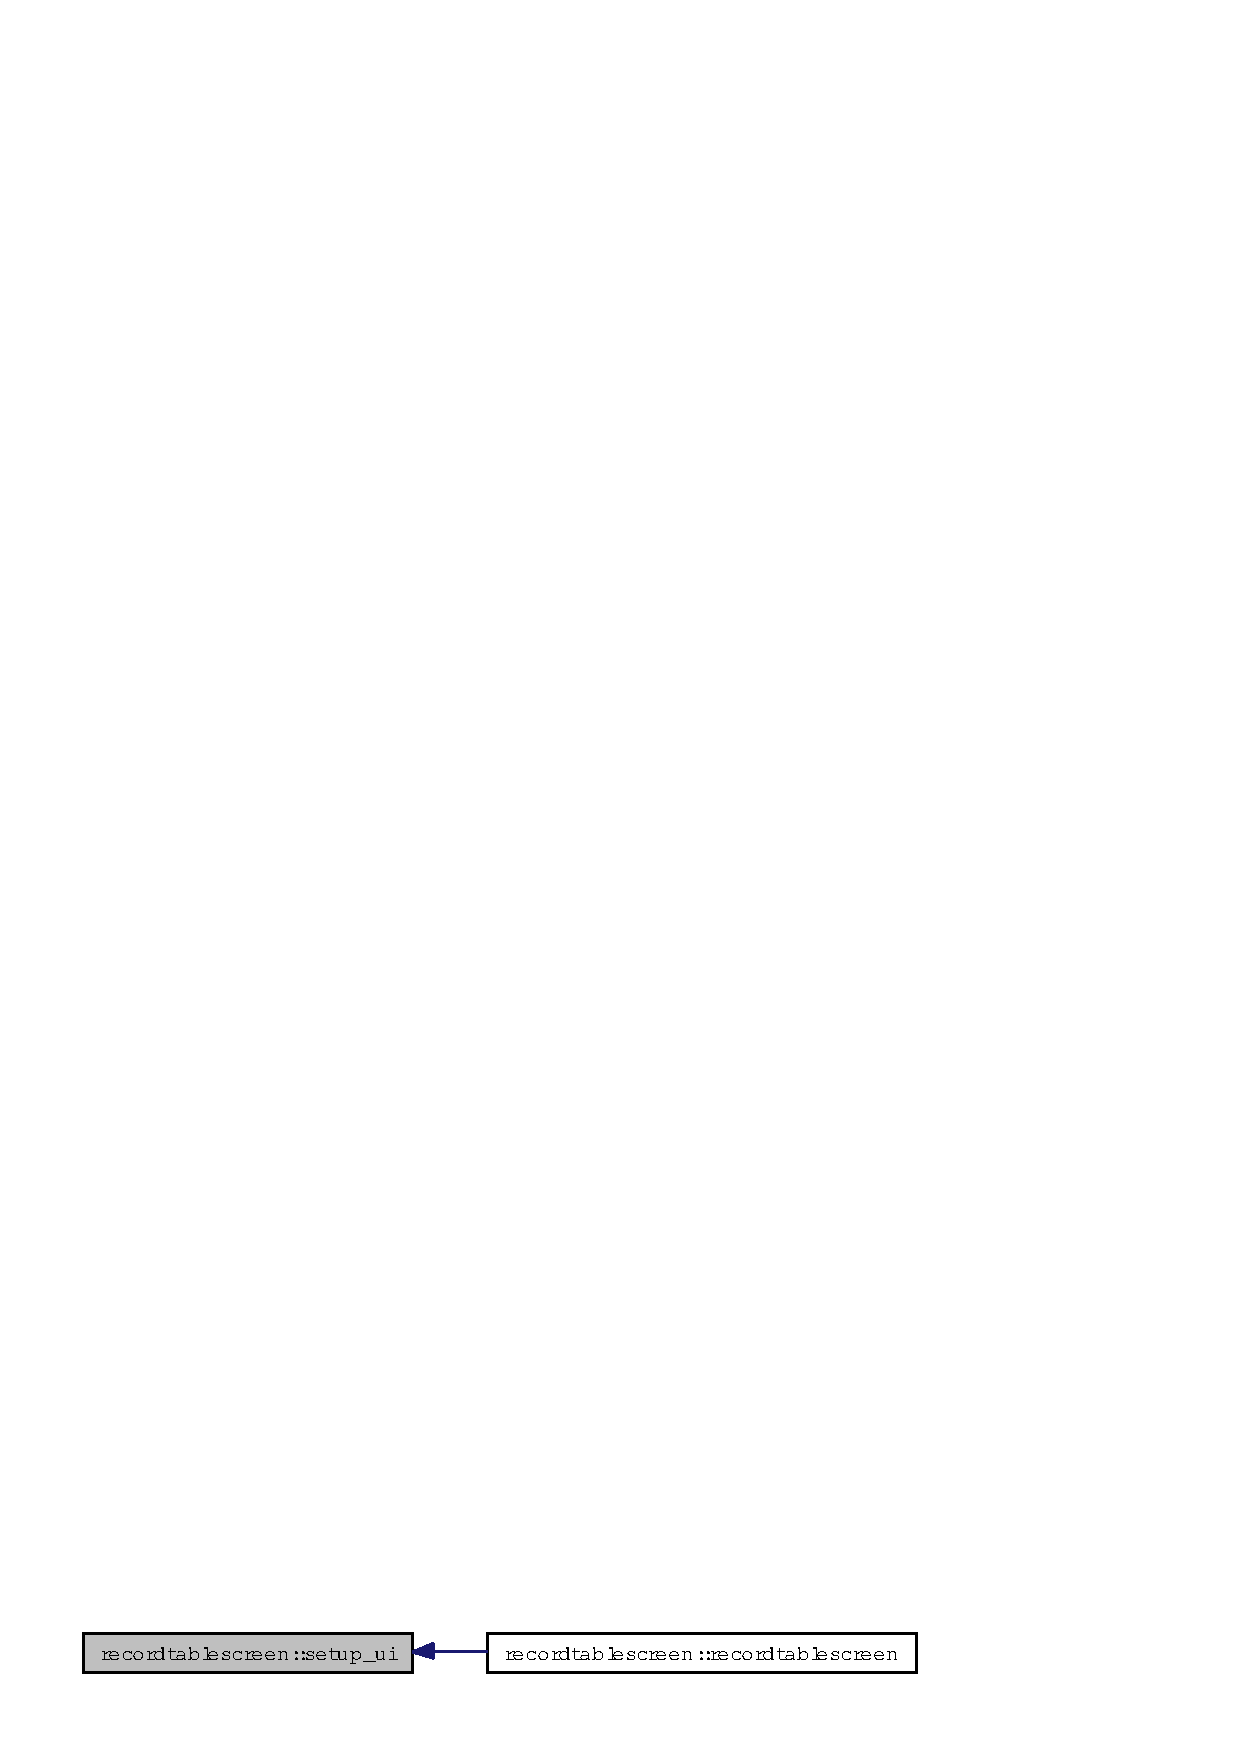
\includegraphics[width=222pt]{classrecordtablescreen_ce88d78bf51cbe1ebeb2515db80dece9_icgraph}
\end{center}
\end{figure}
\index{recordtablescreen@{recordtablescreen}!setup_signals@{setup\_\-signals}}
\index{setup_signals@{setup\_\-signals}!recordtablescreen@{recordtablescreen}}
\subsubsection{\setlength{\rightskip}{0pt plus 5cm}void recordtablescreen::setup\_\-signals (void)\hspace{0.3cm}{\tt  [private]}}\label{classrecordtablescreen_63e5dbd8f4f958c226f79e422b0f17e3}




Definition at line 138 of file recordtablescreen.cpp.

References edit\_\-field\_\-context(), on\_\-custom\-Context\-Menu\-Requested(), recordview, select(), and tools\_\-update().

Referenced by recordtablescreen().

Here is the caller graph for this function:\begin{figure}[H]
\begin{center}
\leavevmode
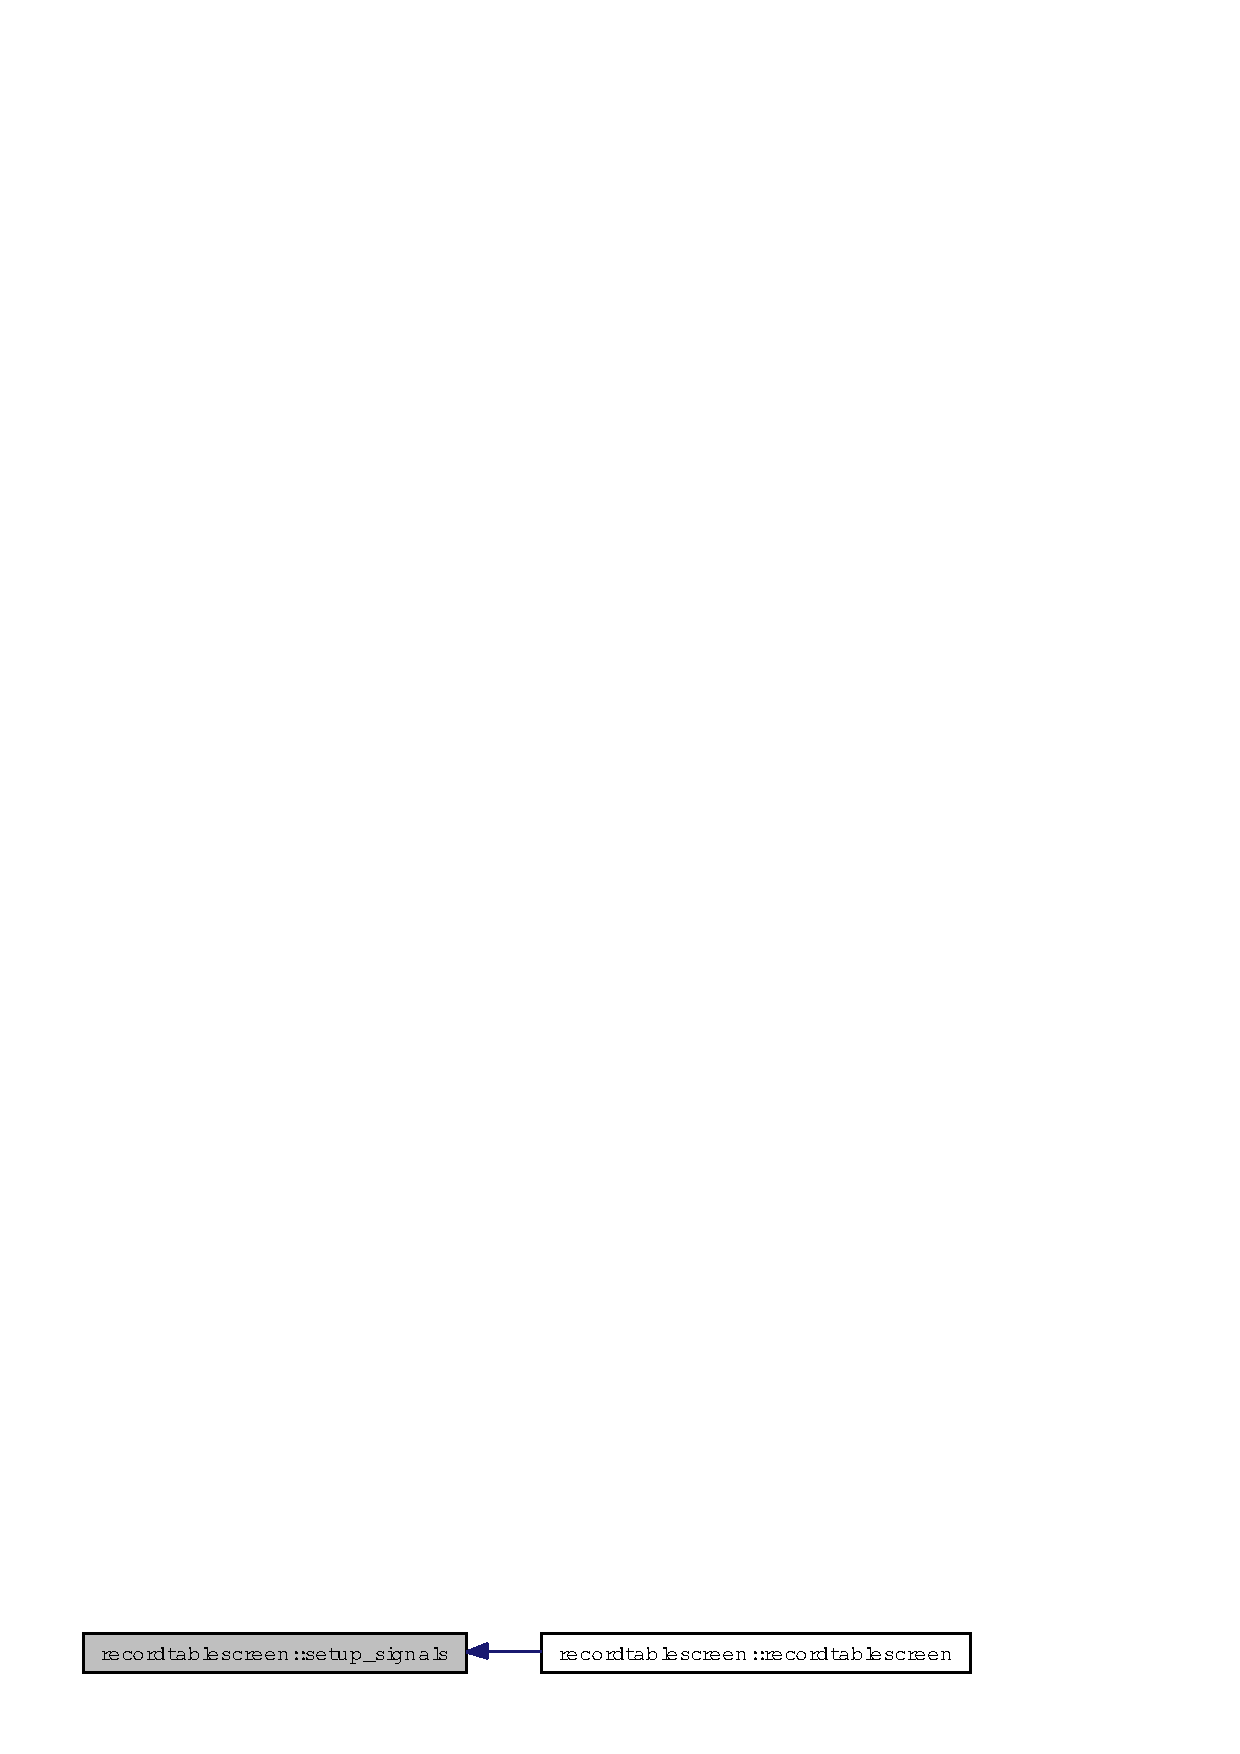
\includegraphics[width=235pt]{classrecordtablescreen_63e5dbd8f4f958c226f79e422b0f17e3_icgraph}
\end{center}
\end{figure}
\index{recordtablescreen@{recordtablescreen}!setup_actions@{setup\_\-actions}}
\index{setup_actions@{setup\_\-actions}!recordtablescreen@{recordtablescreen}}
\subsubsection{\setlength{\rightskip}{0pt plus 5cm}void recordtablescreen::setup\_\-actions (void)\hspace{0.3cm}{\tt  [private]}}\label{classrecordtablescreen_4e8f0ecaef3b8ea55c68ec06386b84ce}




Definition at line 43 of file recordtablescreen.cpp.

References action\_\-add\_\-new\_\-after, action\_\-add\_\-new\_\-before, action\_\-add\_\-new\_\-toend, action\_\-copy, action\_\-cut, action\_\-delete, action\_\-edit\_\-field, action\_\-findinbase, action\_\-movedn, action\_\-moveup, action\_\-paste, add\_\-new\_\-after\_\-context(), add\_\-new\_\-before\_\-context(), add\_\-new\_\-toend\_\-context(), copy(), cut(), delete\_\-context(), disable\_\-all\_\-actions(), edit\_\-field\_\-context(), findinbase\_\-open(), movedn(), moveup(), and paste().

Referenced by recordtablescreen().

Here is the call graph for this function:\begin{figure}[H]
\begin{center}
\leavevmode
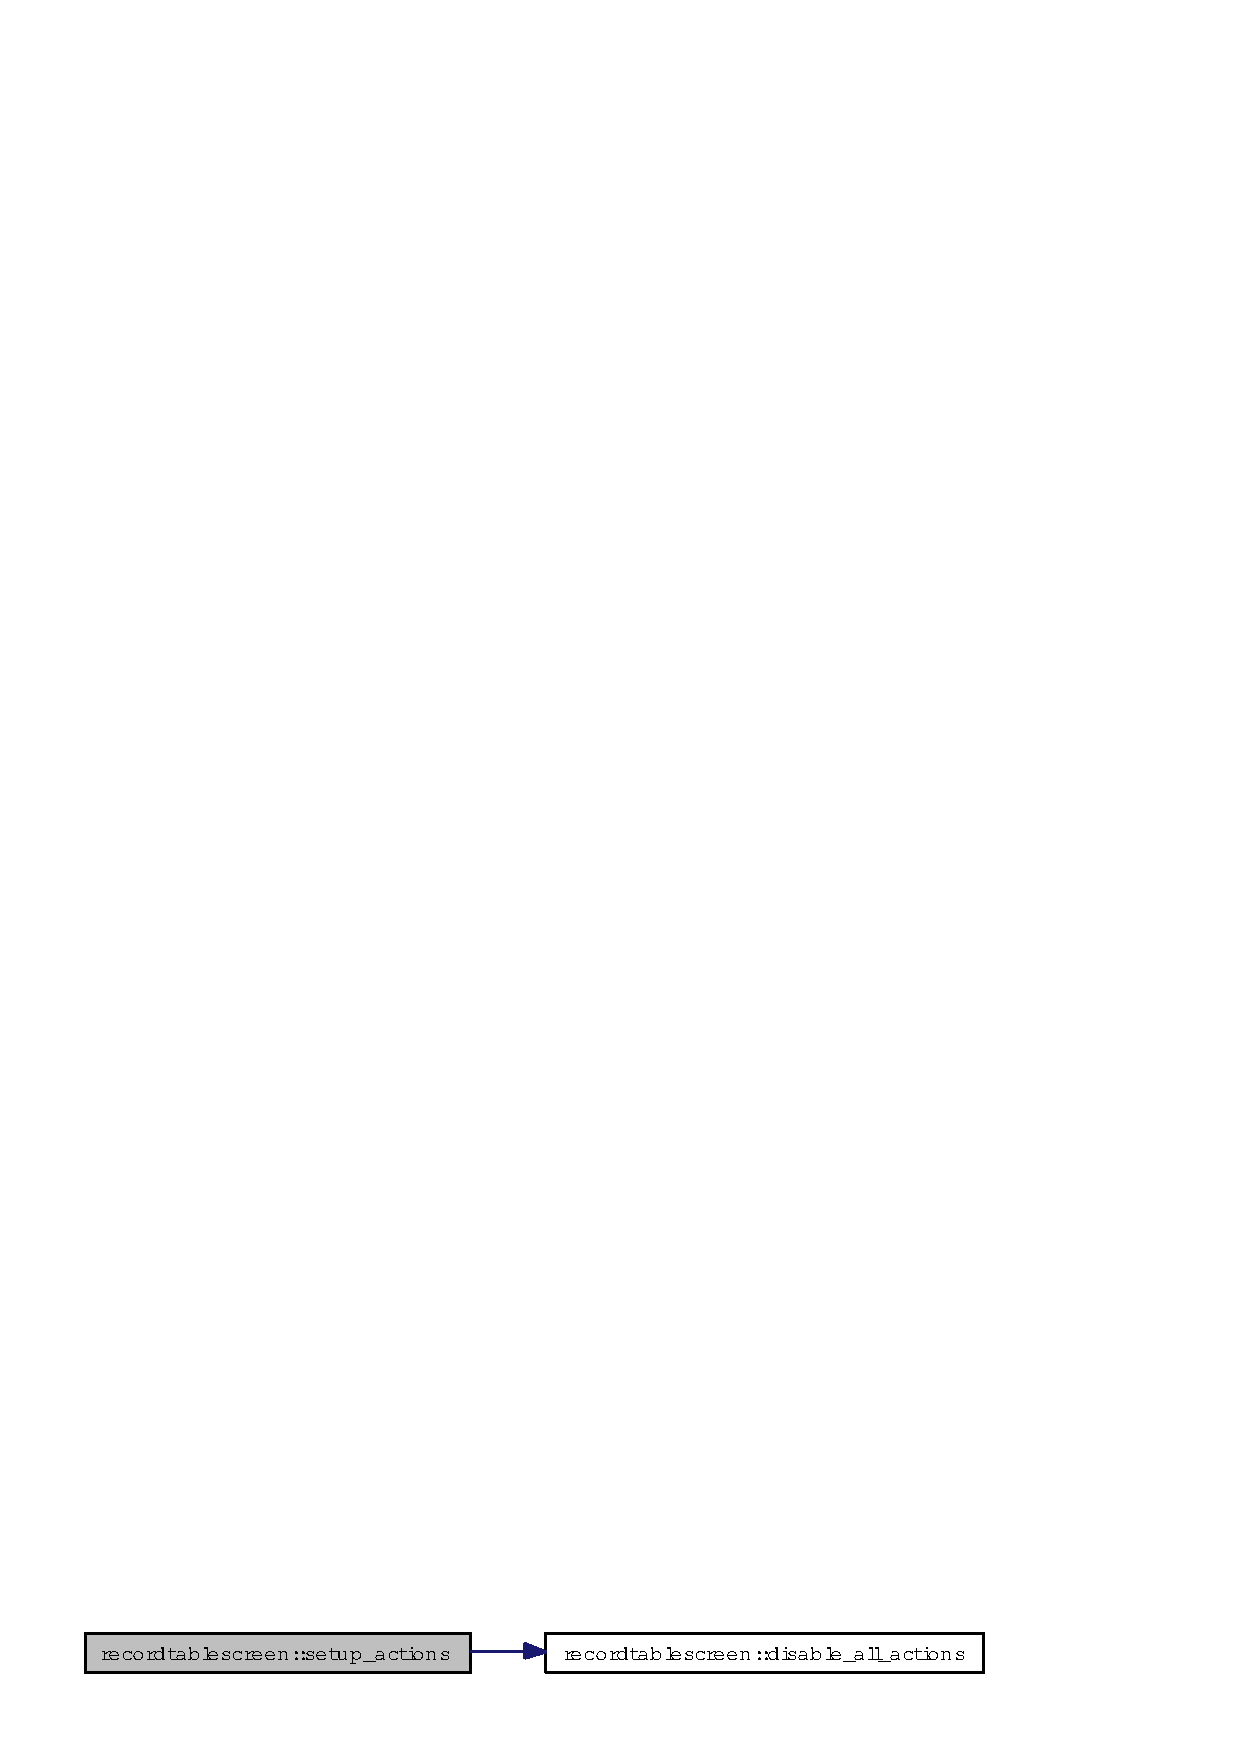
\includegraphics[width=238pt]{classrecordtablescreen_4e8f0ecaef3b8ea55c68ec06386b84ce_cgraph}
\end{center}
\end{figure}


Here is the caller graph for this function:\begin{figure}[H]
\begin{center}
\leavevmode
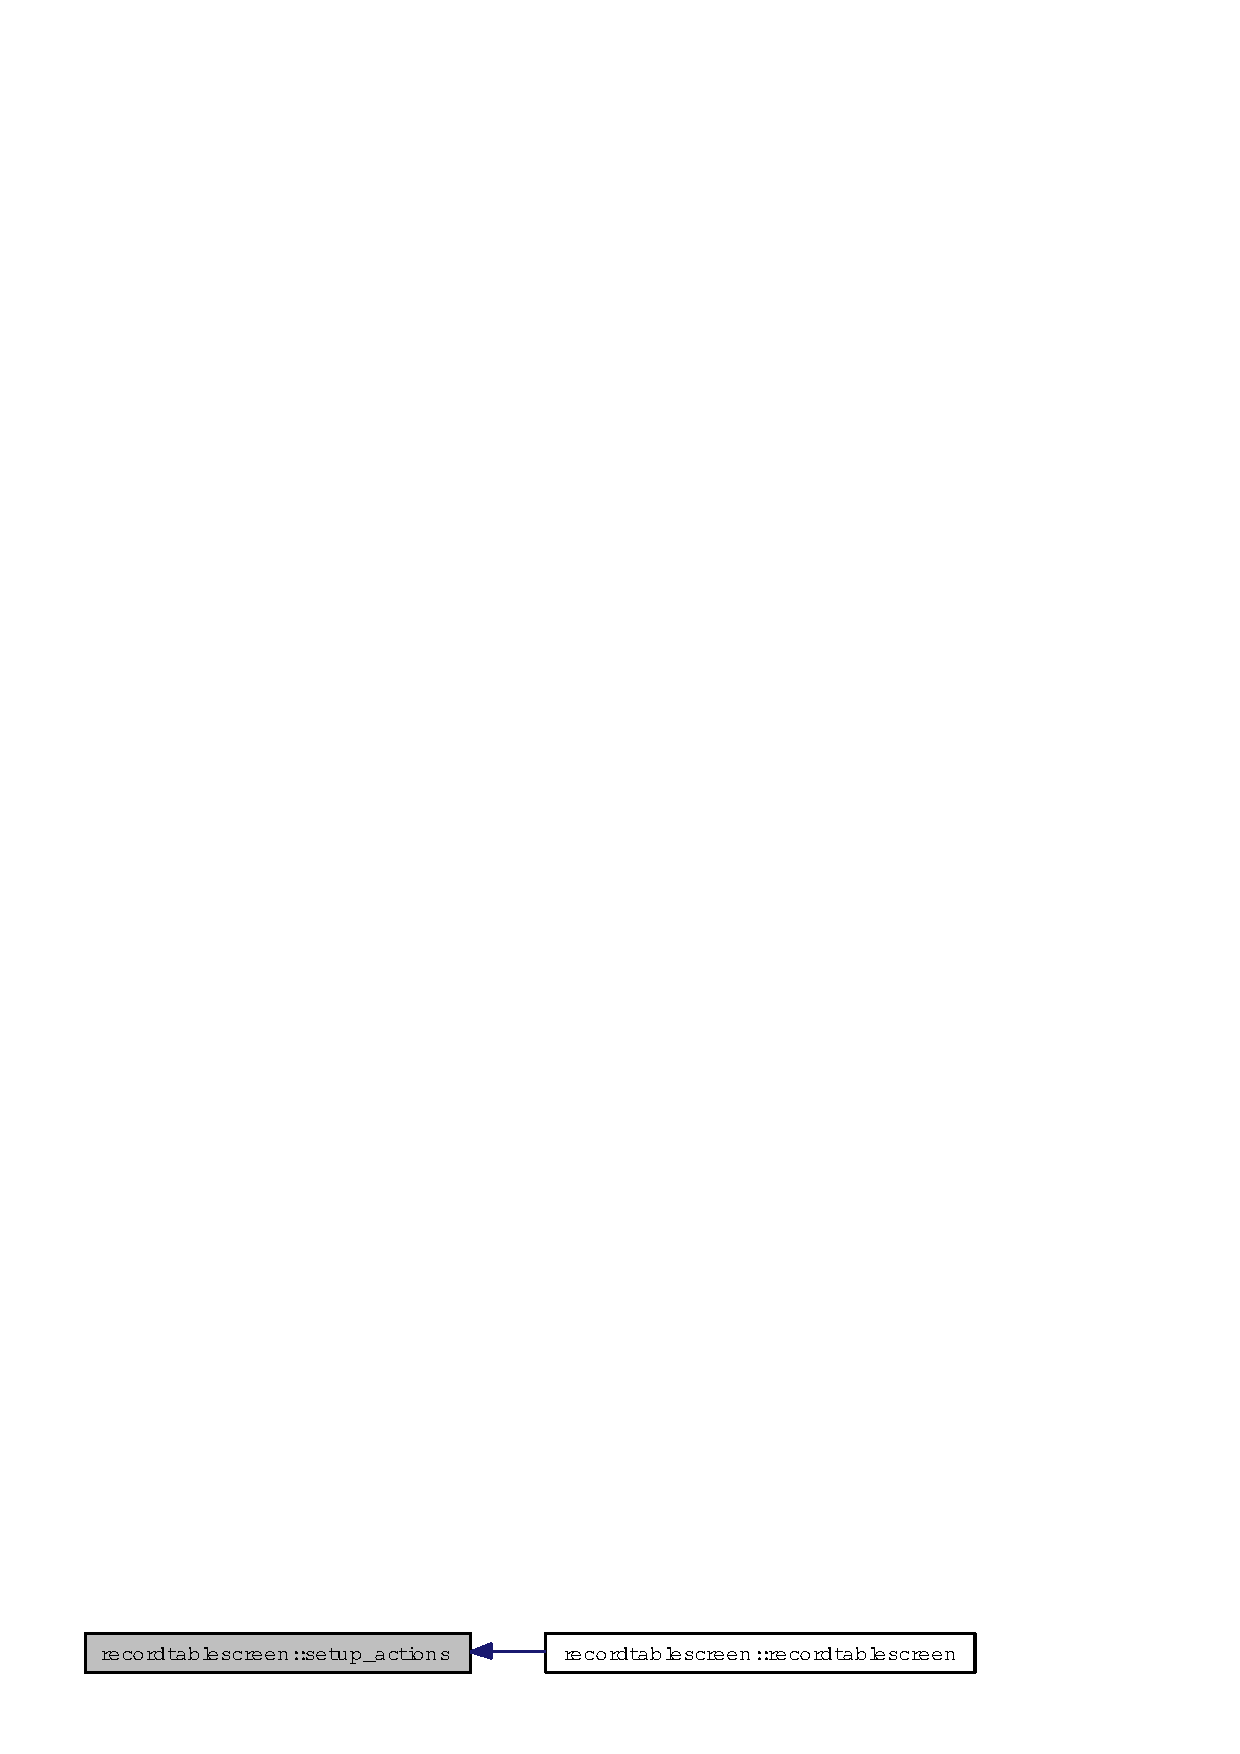
\includegraphics[width=236pt]{classrecordtablescreen_4e8f0ecaef3b8ea55c68ec06386b84ce_icgraph}
\end{center}
\end{figure}
\index{recordtablescreen@{recordtablescreen}!assembly@{assembly}}
\index{assembly@{assembly}!recordtablescreen@{recordtablescreen}}
\subsubsection{\setlength{\rightskip}{0pt plus 5cm}void recordtablescreen::assembly (void)\hspace{0.3cm}{\tt  [private]}}\label{classrecordtablescreen_ed6b3c5241560d8599f657586fe32b2b}




Definition at line 174 of file recordtablescreen.cpp.

References find\_\-line, recordtable\_\-tools\_\-layout, recordtablescreen\_\-layout, recordview, and tools\_\-line.

Referenced by recordtablescreen().

Here is the caller graph for this function:\begin{figure}[H]
\begin{center}
\leavevmode
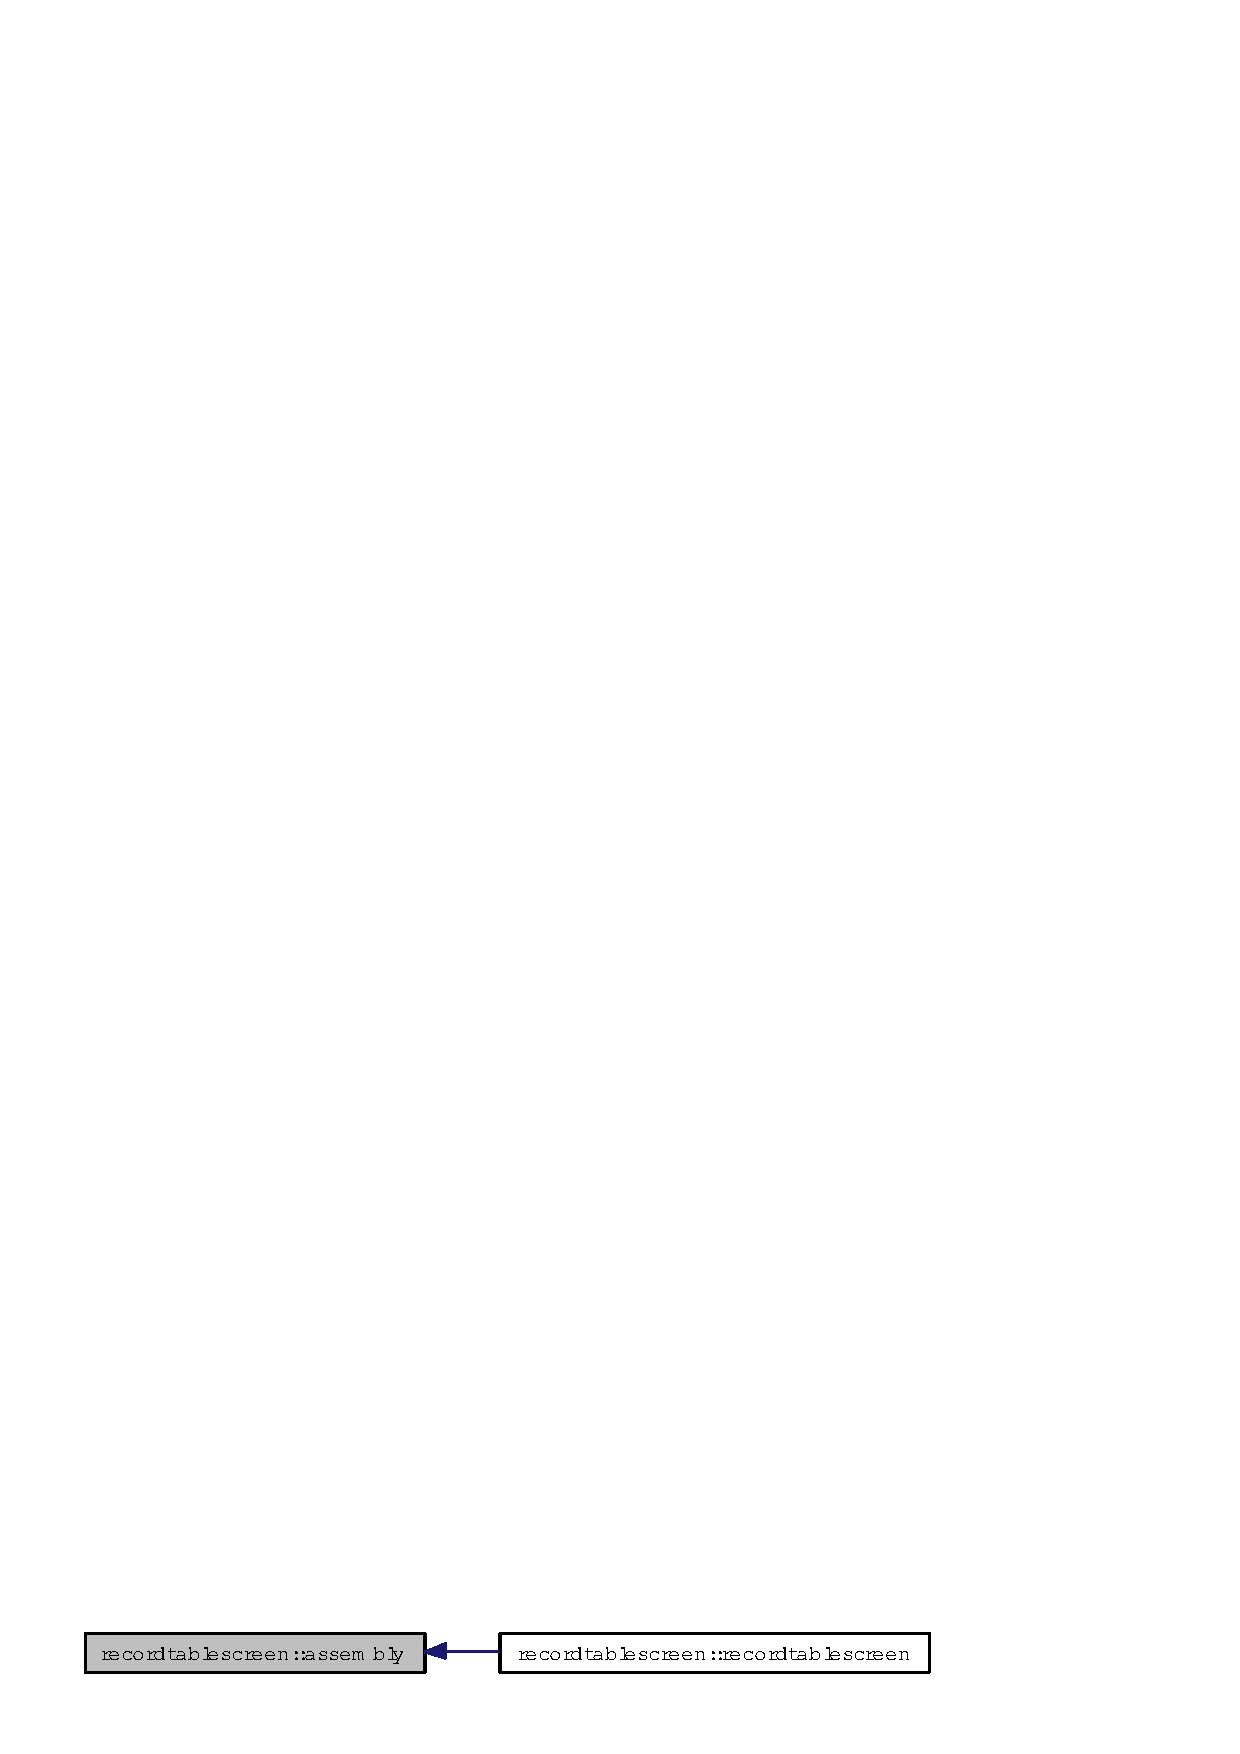
\includegraphics[width=225pt]{classrecordtablescreen_ed6b3c5241560d8599f657586fe32b2b_icgraph}
\end{center}
\end{figure}
\index{recordtablescreen@{recordtablescreen}!disable_all_actions@{disable\_\-all\_\-actions}}
\index{disable_all_actions@{disable\_\-all\_\-actions}!recordtablescreen@{recordtablescreen}}
\subsubsection{\setlength{\rightskip}{0pt plus 5cm}void recordtablescreen::disable\_\-all\_\-actions (void)\hspace{0.3cm}{\tt  [private]}}\label{classrecordtablescreen_29e17faab1f97b595f897d80c287f92d}




Definition at line 640 of file recordtablescreen.cpp.

References action\_\-add\_\-new\_\-after, action\_\-add\_\-new\_\-before, action\_\-add\_\-new\_\-toend, action\_\-copy, action\_\-cut, action\_\-delete, action\_\-edit\_\-field, action\_\-movedn, action\_\-moveup, and action\_\-paste.

Referenced by setup\_\-actions(), and tools\_\-update().

Here is the caller graph for this function:\begin{figure}[H]
\begin{center}
\leavevmode
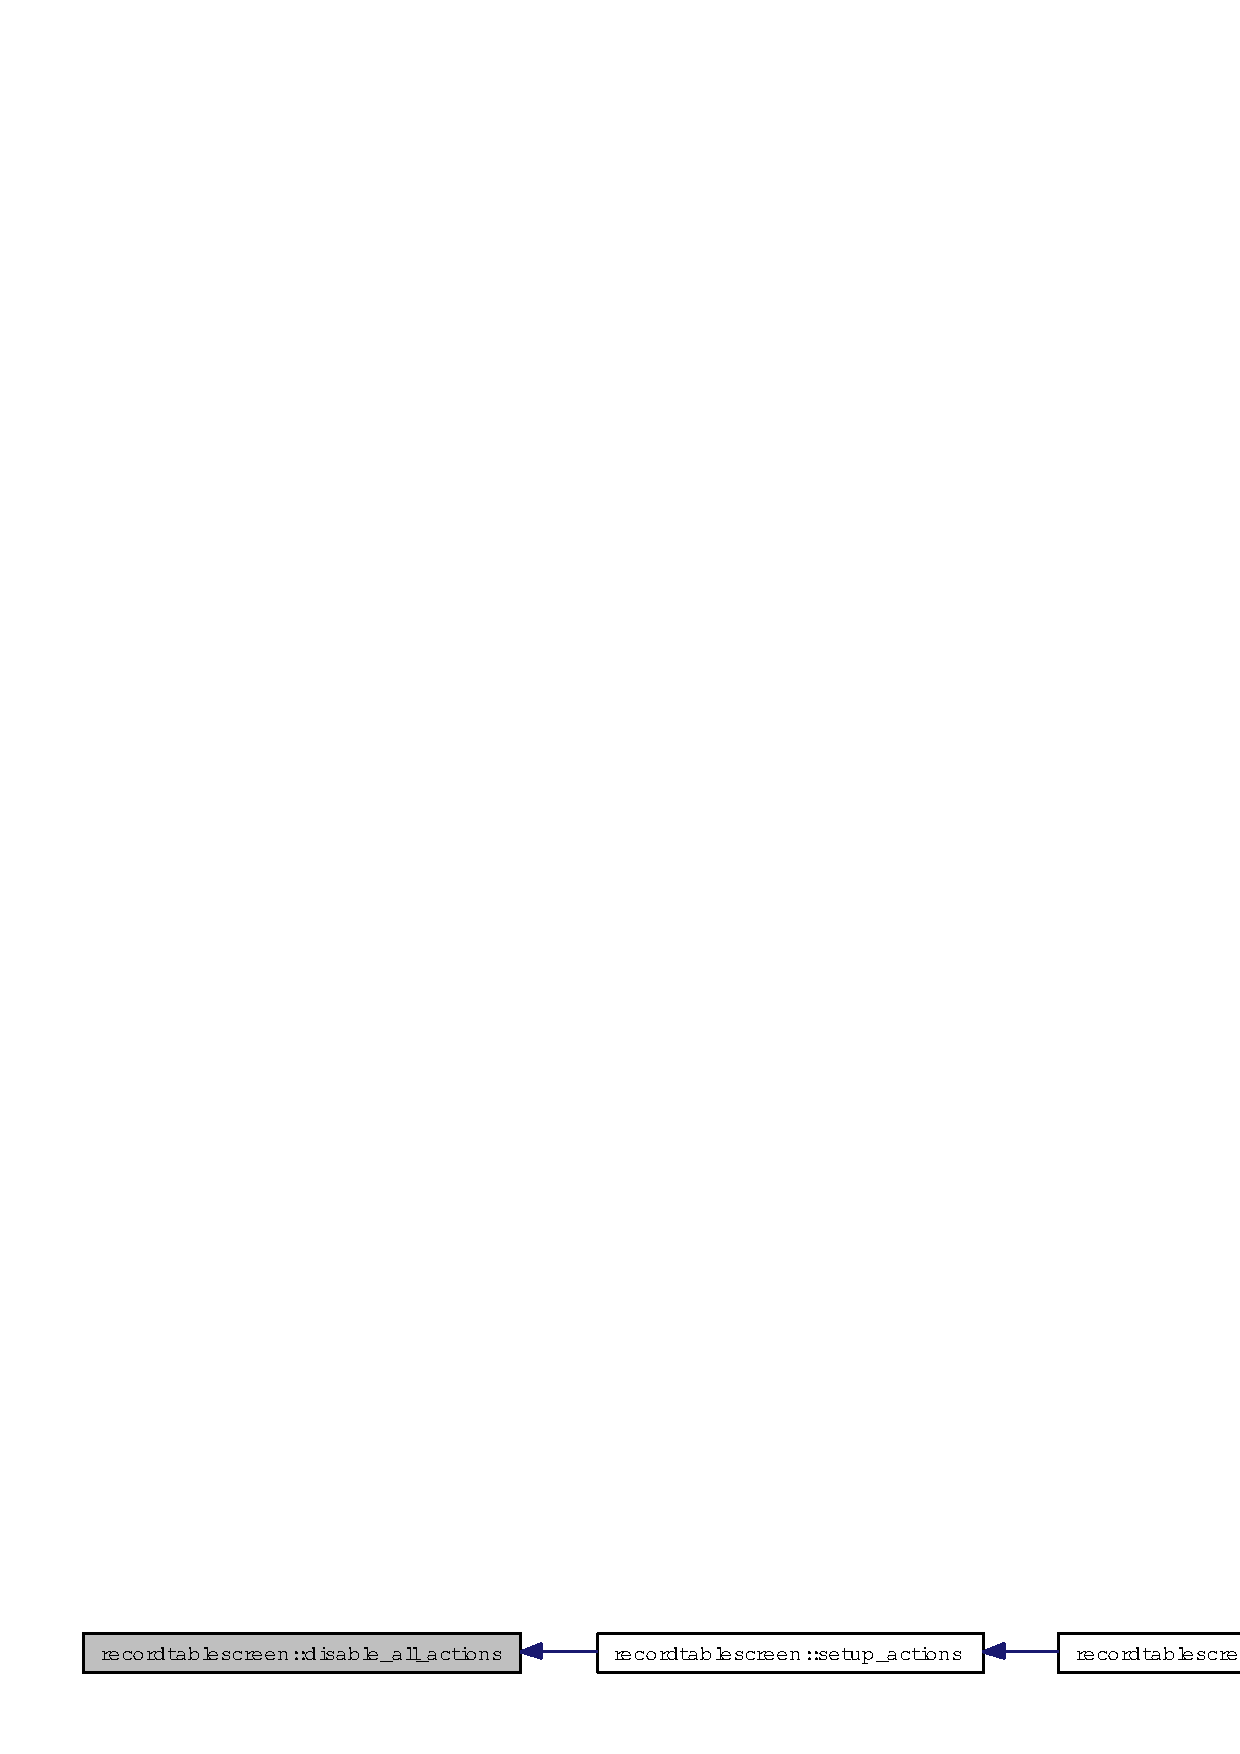
\includegraphics[width=359pt]{classrecordtablescreen_29e17faab1f97b595f897d80c287f92d_icgraph}
\end{center}
\end{figure}
\index{recordtablescreen@{recordtablescreen}!add_new_record@{add\_\-new\_\-record}}
\index{add_new_record@{add\_\-new\_\-record}!recordtablescreen@{recordtablescreen}}
\subsubsection{\setlength{\rightskip}{0pt plus 5cm}void recordtablescreen::add\_\-new\_\-record (int {\em mode})\hspace{0.3cm}{\tt  [private]}}\label{classrecordtablescreen_e52ce4d7625ab4d1a78938b3028652be}




Definition at line 329 of file recordtablescreen.cpp.

References add\_\-new(), and addnewrecord::get\_\-field().

Referenced by add\_\-new\_\-after\_\-context(), add\_\-new\_\-before\_\-context(), and add\_\-new\_\-toend\_\-context().

Here is the call graph for this function:\begin{figure}[H]
\begin{center}
\leavevmode
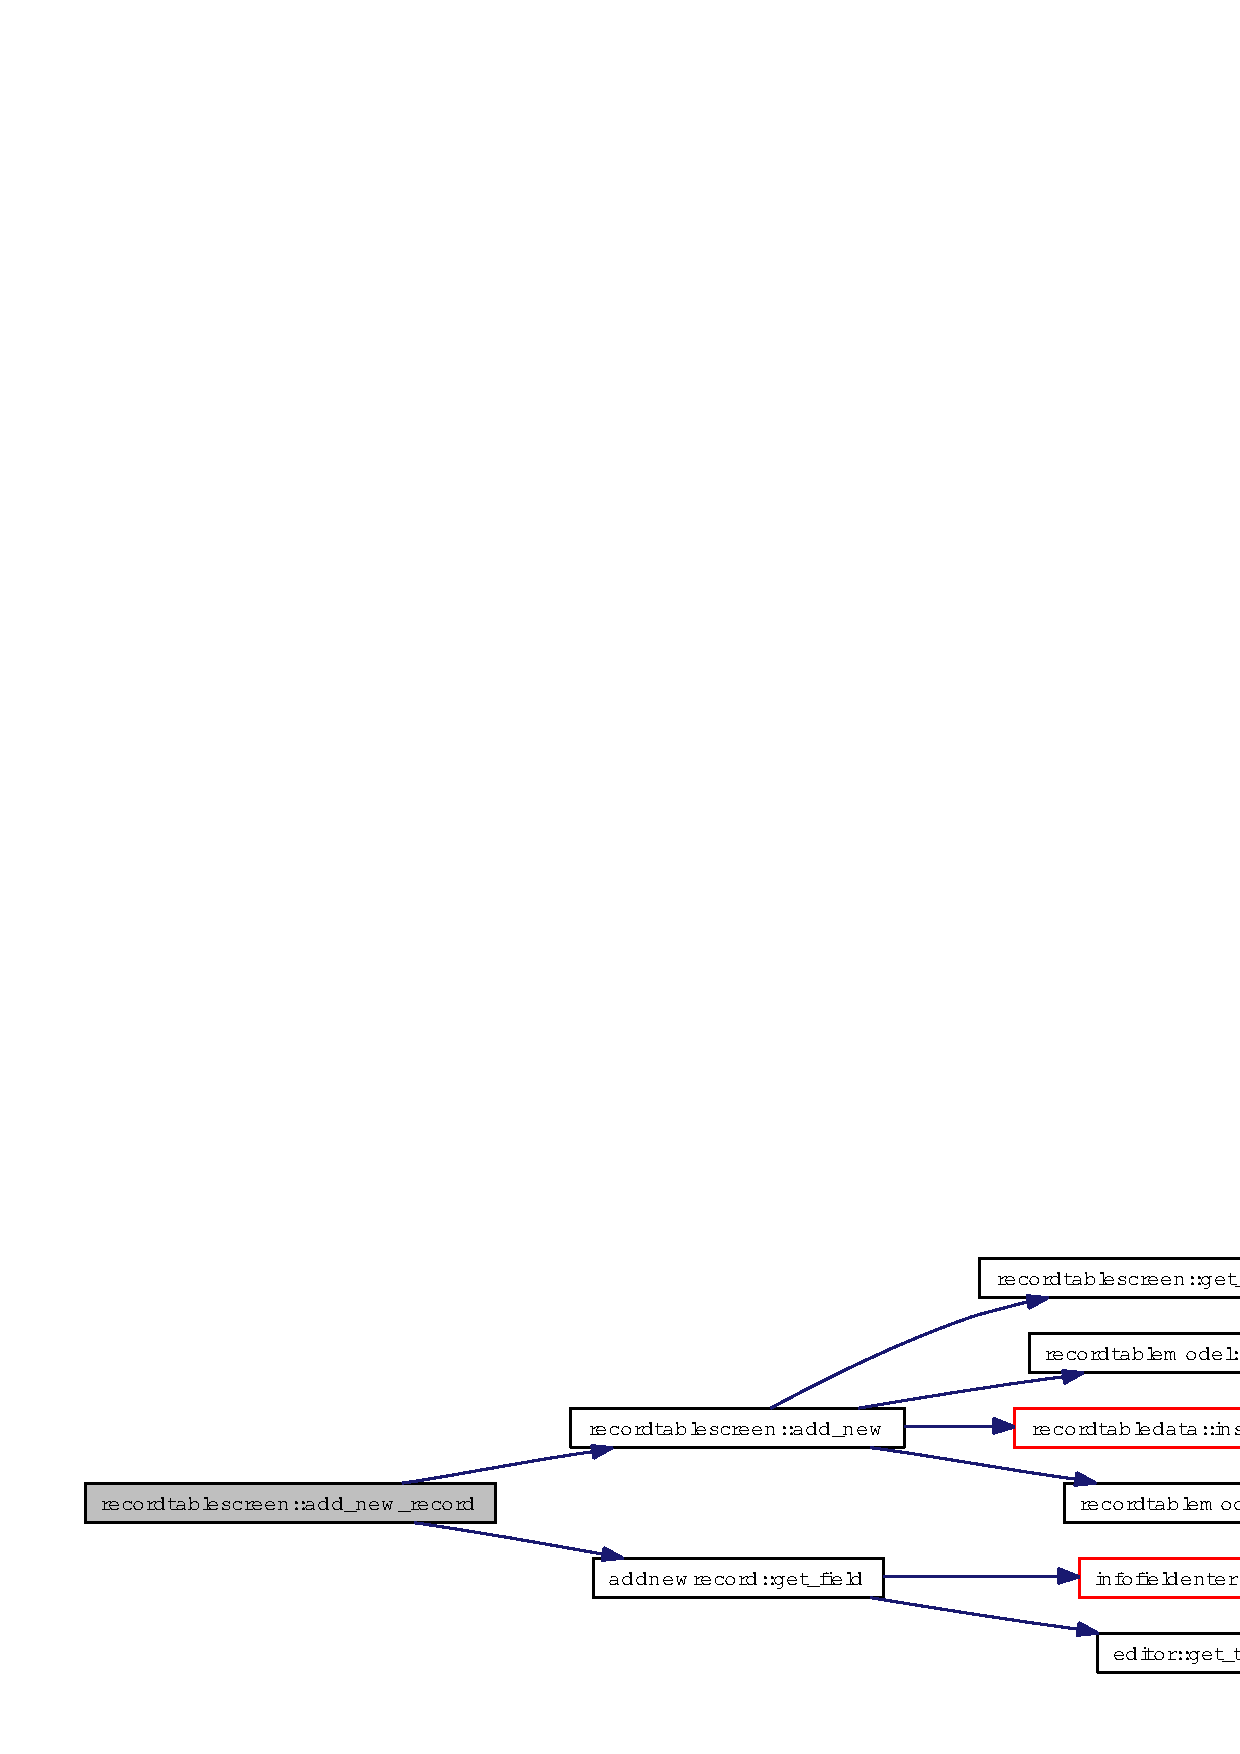
\includegraphics[width=352pt]{classrecordtablescreen_e52ce4d7625ab4d1a78938b3028652be_cgraph}
\end{center}
\end{figure}
\index{recordtablescreen@{recordtablescreen}!add_new@{add\_\-new}}
\index{add_new@{add\_\-new}!recordtablescreen@{recordtablescreen}}
\subsubsection{\setlength{\rightskip}{0pt plus 5cm}void recordtablescreen::add\_\-new (int {\em mode}, QString {\em name}, QString {\em author}, QString {\em url}, QString {\em tags}, QString {\em text})\hspace{0.3cm}{\tt  [private]}}\label{classrecordtablescreen_e3e3b5770bfdb550262ff4dab723599a}




Definition at line 349 of file recordtablescreen.cpp.

References get\_\-first\_\-selection\_\-pos(), recordtablemodel::get\_\-tabledata(), recordtabledata::insert\_\-new\_\-record(), recordmodel, recordview, and recordtablemodel::update().

Referenced by add\_\-new\_\-record(), and paste().

Here is the call graph for this function:\begin{figure}[H]
\begin{center}
\leavevmode
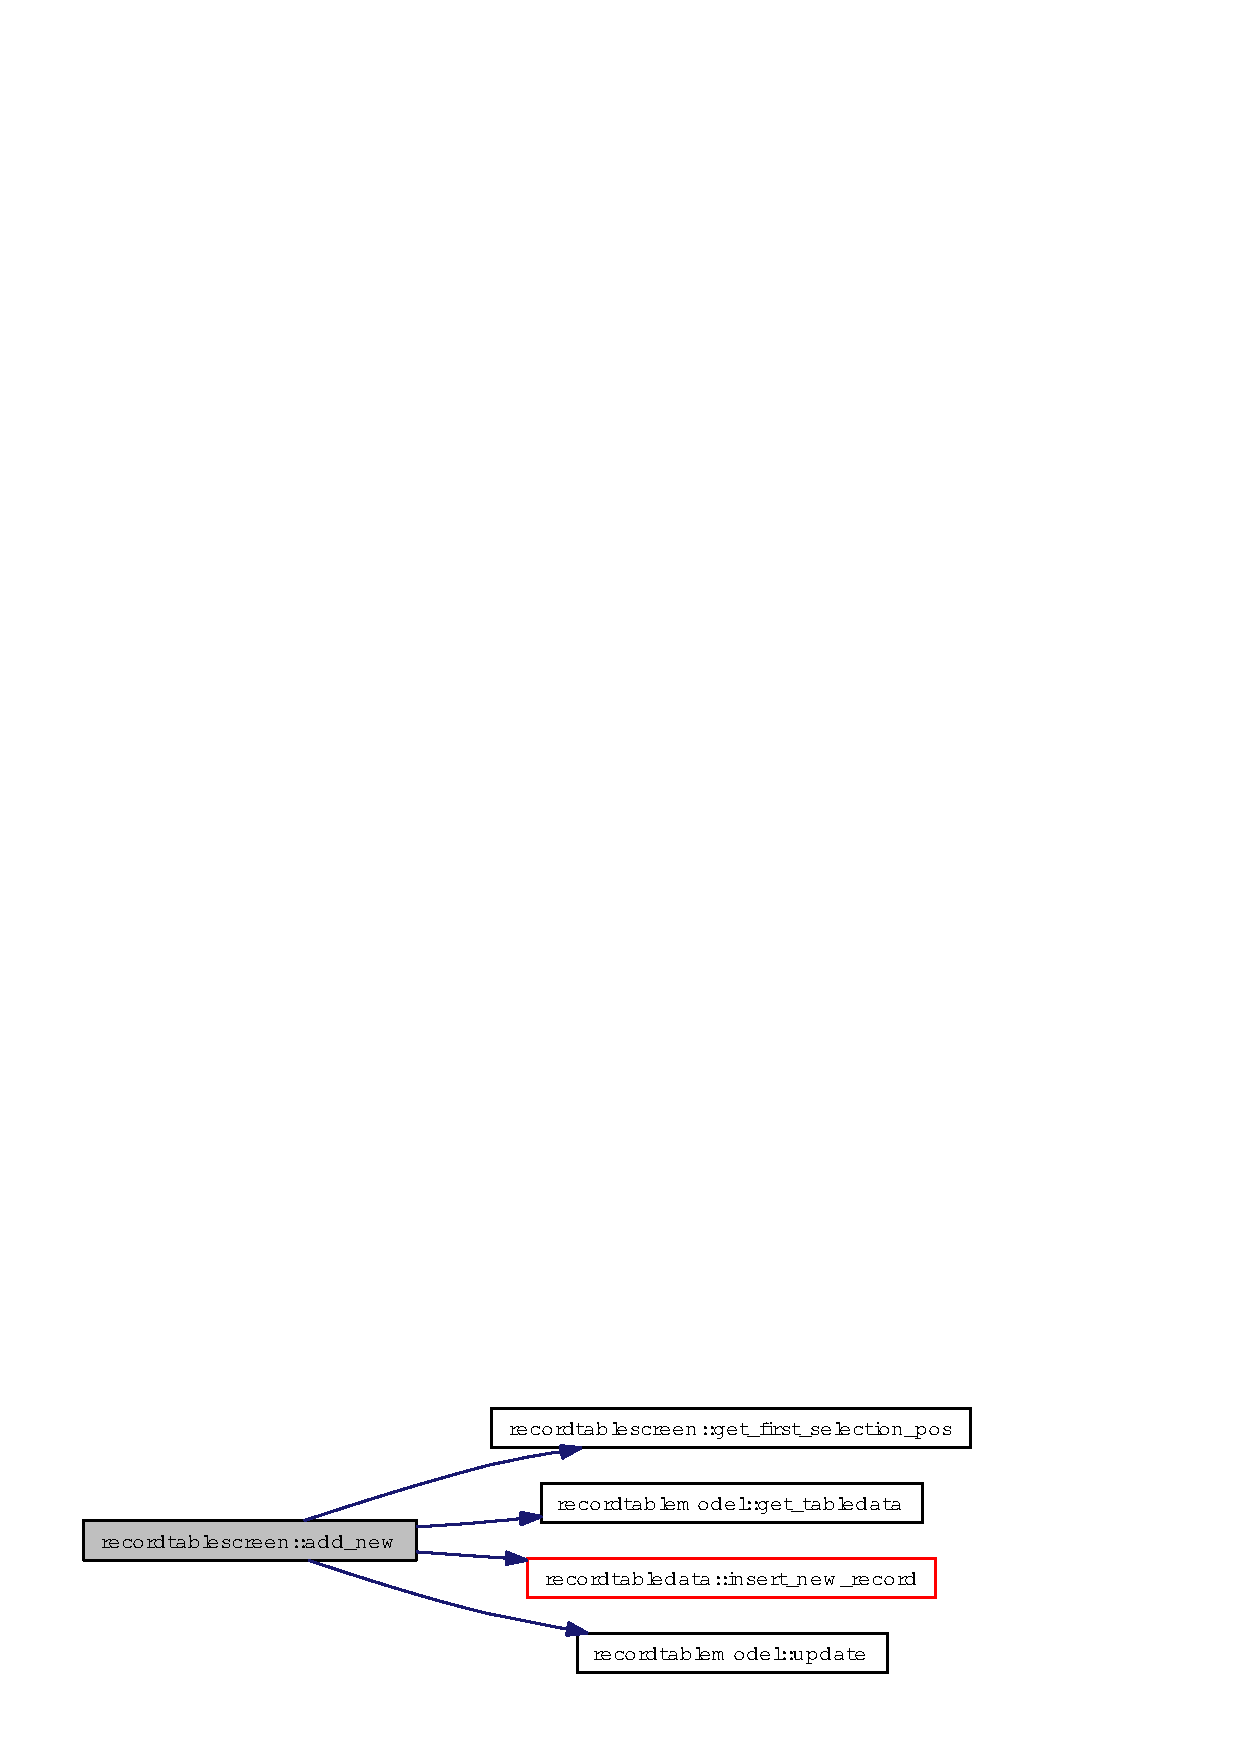
\includegraphics[width=235pt]{classrecordtablescreen_e3e3b5770bfdb550262ff4dab723599a_cgraph}
\end{center}
\end{figure}


Here is the caller graph for this function:\begin{figure}[H]
\begin{center}
\leavevmode
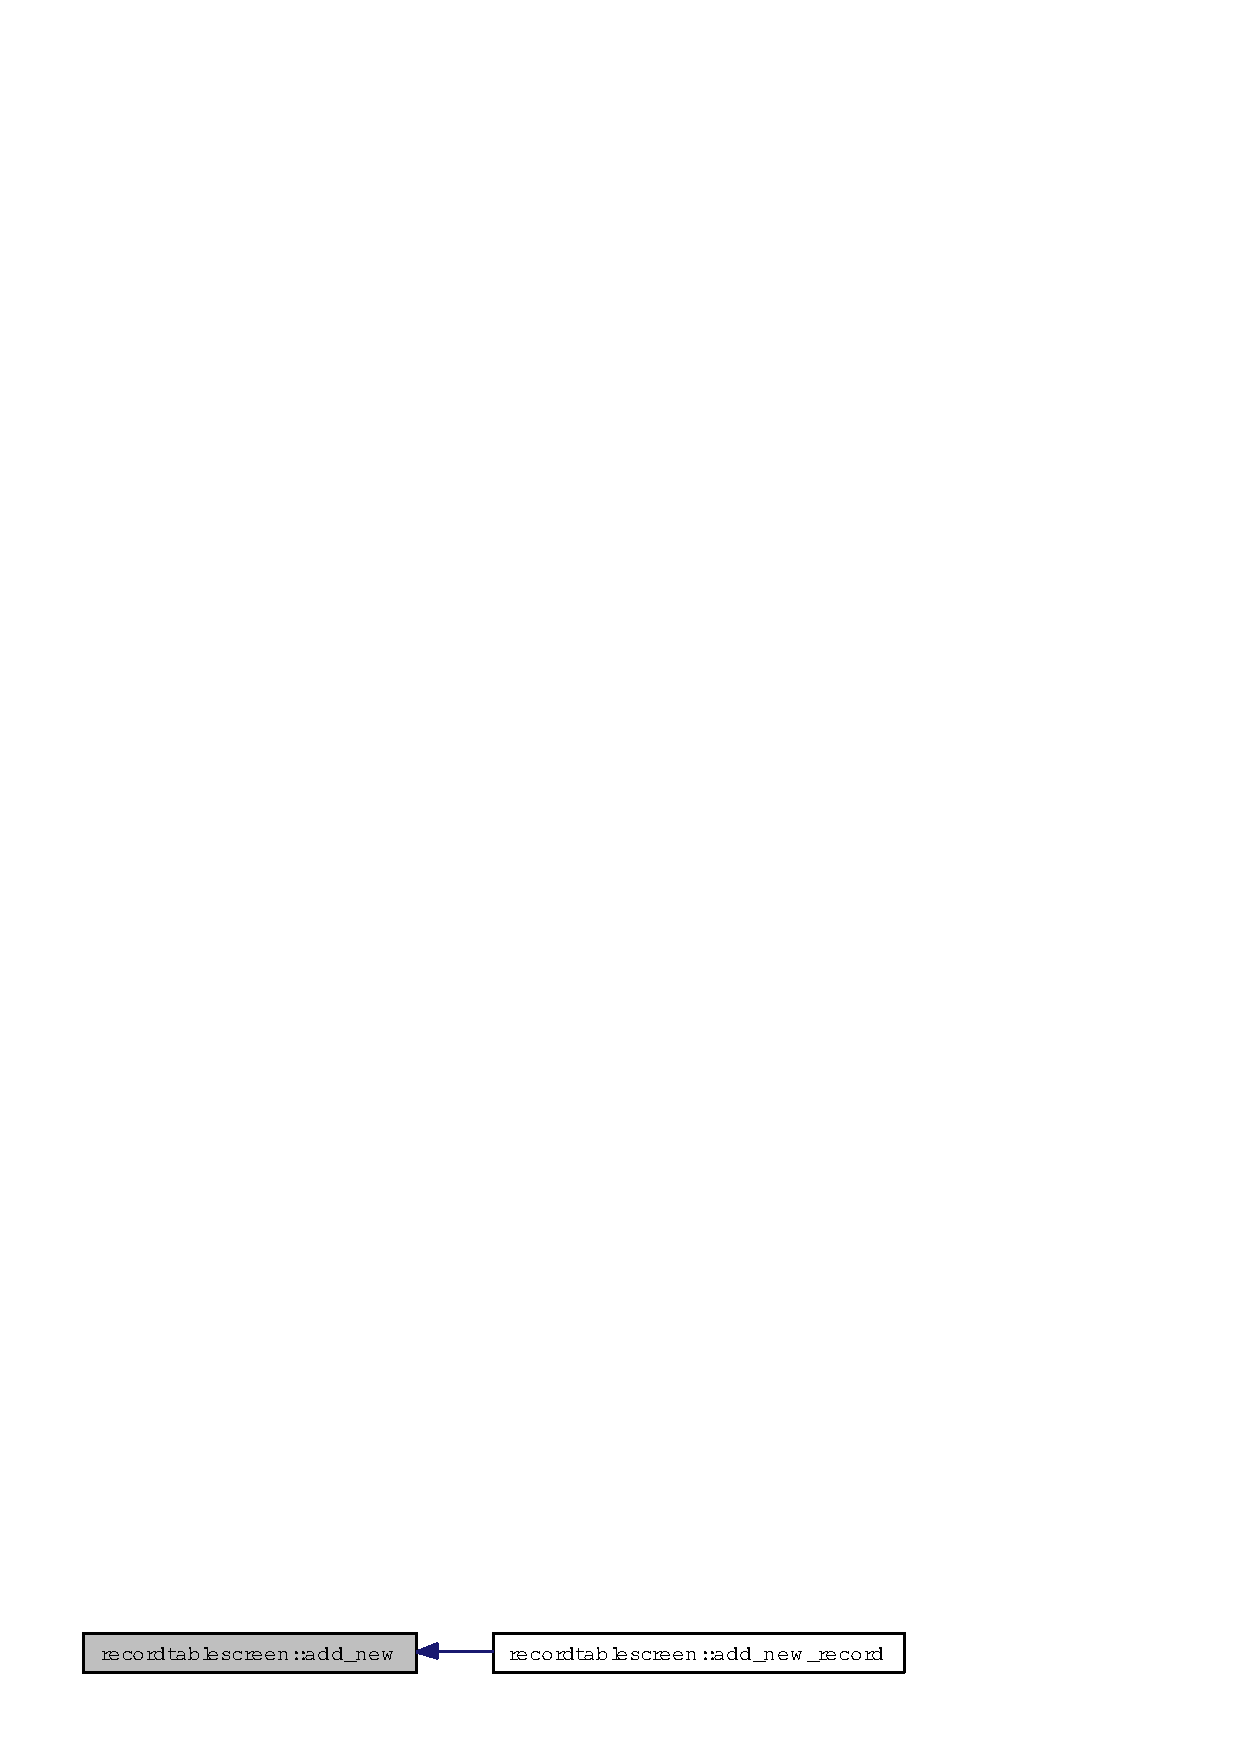
\includegraphics[width=219pt]{classrecordtablescreen_e3e3b5770bfdb550262ff4dab723599a_icgraph}
\end{center}
\end{figure}
\index{recordtablescreen@{recordtablescreen}!edit_field@{edit\_\-field}}
\index{edit_field@{edit\_\-field}!recordtablescreen@{recordtablescreen}}
\subsubsection{\setlength{\rightskip}{0pt plus 5cm}void recordtablescreen::edit\_\-field (int {\em pos}, QString {\em name}, QString {\em author}, QString {\em url}, QString {\em tags})\hspace{0.3cm}{\tt  [private]}}\label{classrecordtablescreen_41863650780dd07b0fc1275f748f78b4}




Definition at line 424 of file recordtablescreen.cpp.

References recordtabledata::edit\_\-record(), recordtablemodel::get\_\-tabledata(), recordmodel, metaeditor::set\_\-author(), metaeditor::set\_\-name(), metaeditor::set\_\-tags(), and metaeditor::set\_\-url().

Referenced by edit\_\-field\_\-context().

Here is the call graph for this function:\begin{figure}[H]
\begin{center}
\leavevmode
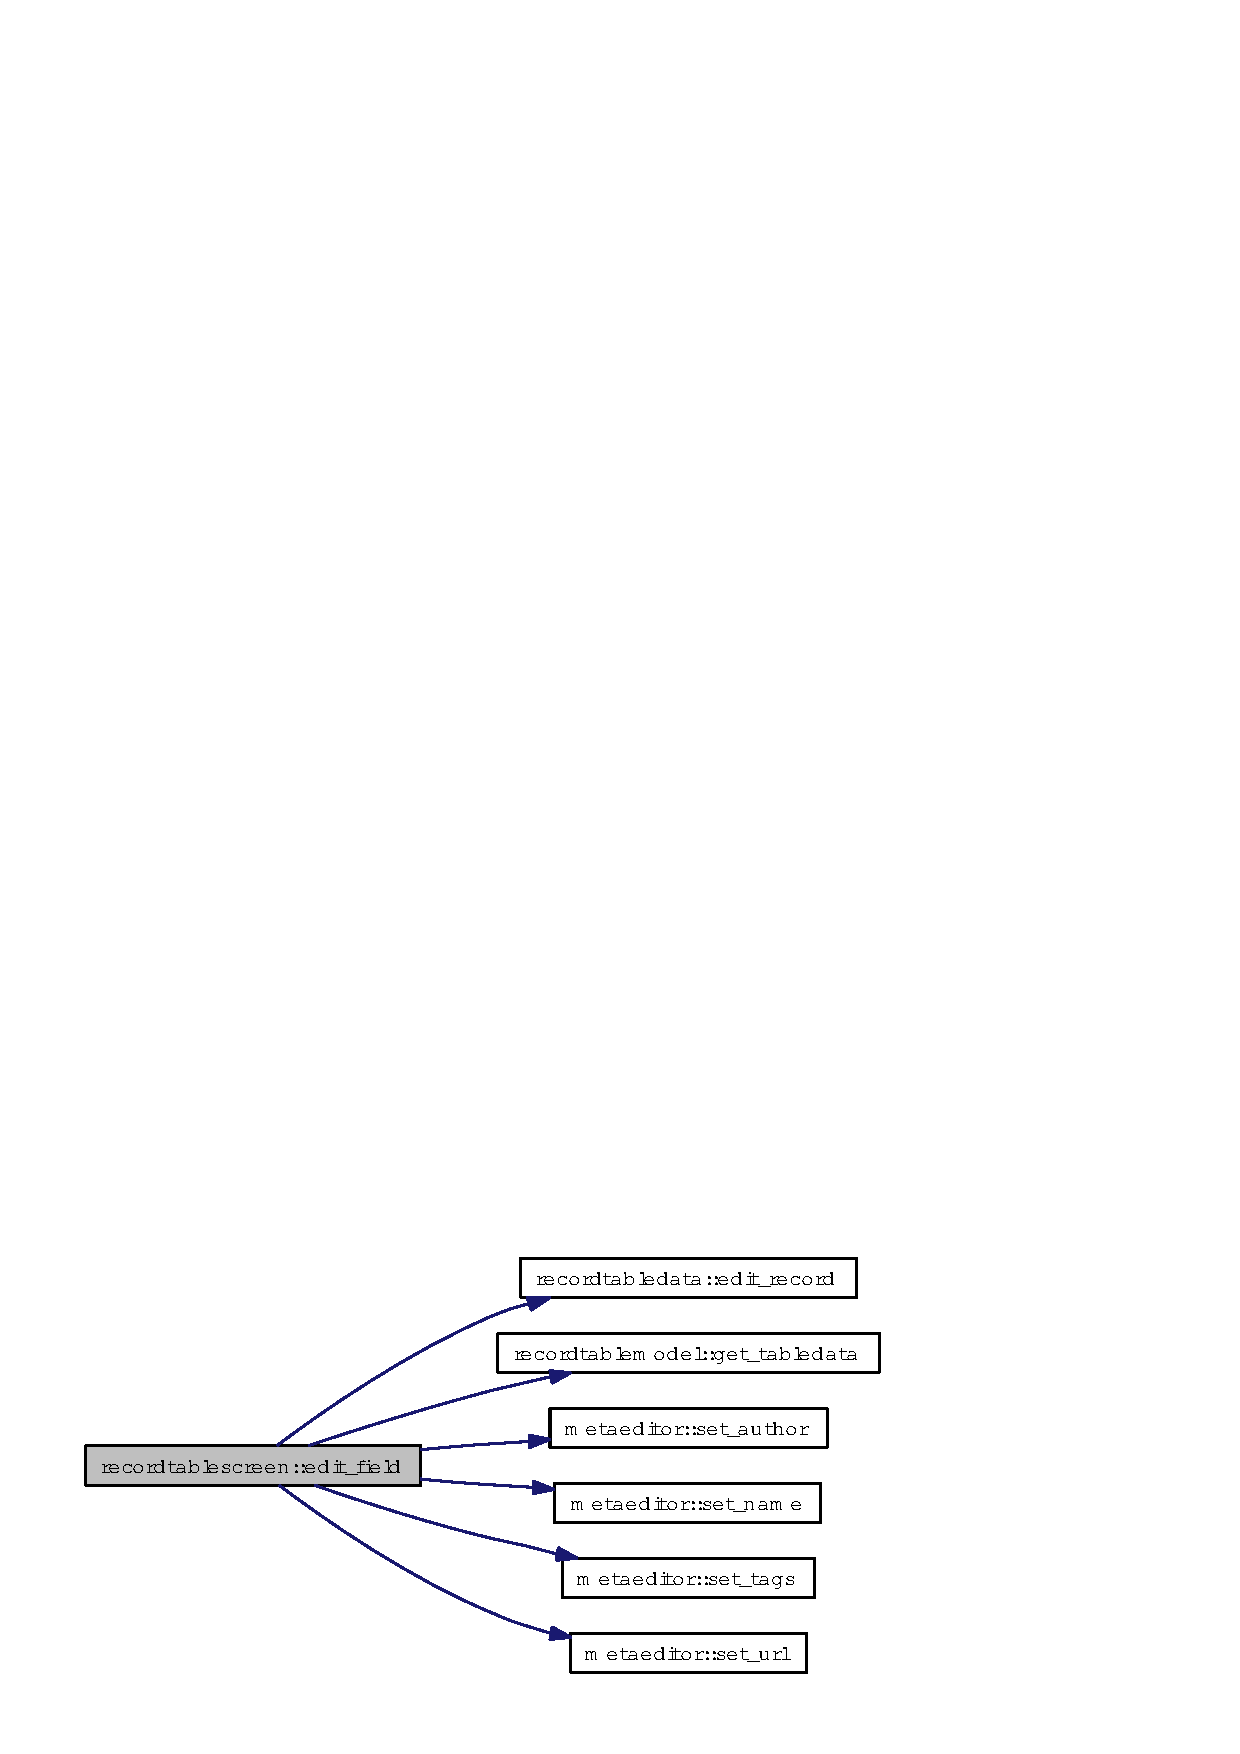
\includegraphics[width=213pt]{classrecordtablescreen_41863650780dd07b0fc1275f748f78b4_cgraph}
\end{center}
\end{figure}
\index{recordtablescreen@{recordtablescreen}!delete_records@{delete\_\-records}}
\index{delete_records@{delete\_\-records}!recordtablescreen@{recordtablescreen}}
\subsubsection{\setlength{\rightskip}{0pt plus 5cm}void recordtablescreen::delete\_\-records (void)\hspace{0.3cm}{\tt  [private]}}\label{classrecordtablescreen_91d1bc4b540ad9af78437a59143e94a4}




Definition at line 476 of file recordtablescreen.cpp.

References recordtabledata::delete\_\-records(), recordtablemodel::get\_\-tabledata(), recordmodel, recordview, recordtabledata::size(), and recordtablemodel::update().

Referenced by cut(), and delete\_\-context().

Here is the call graph for this function:\begin{figure}[H]
\begin{center}
\leavevmode
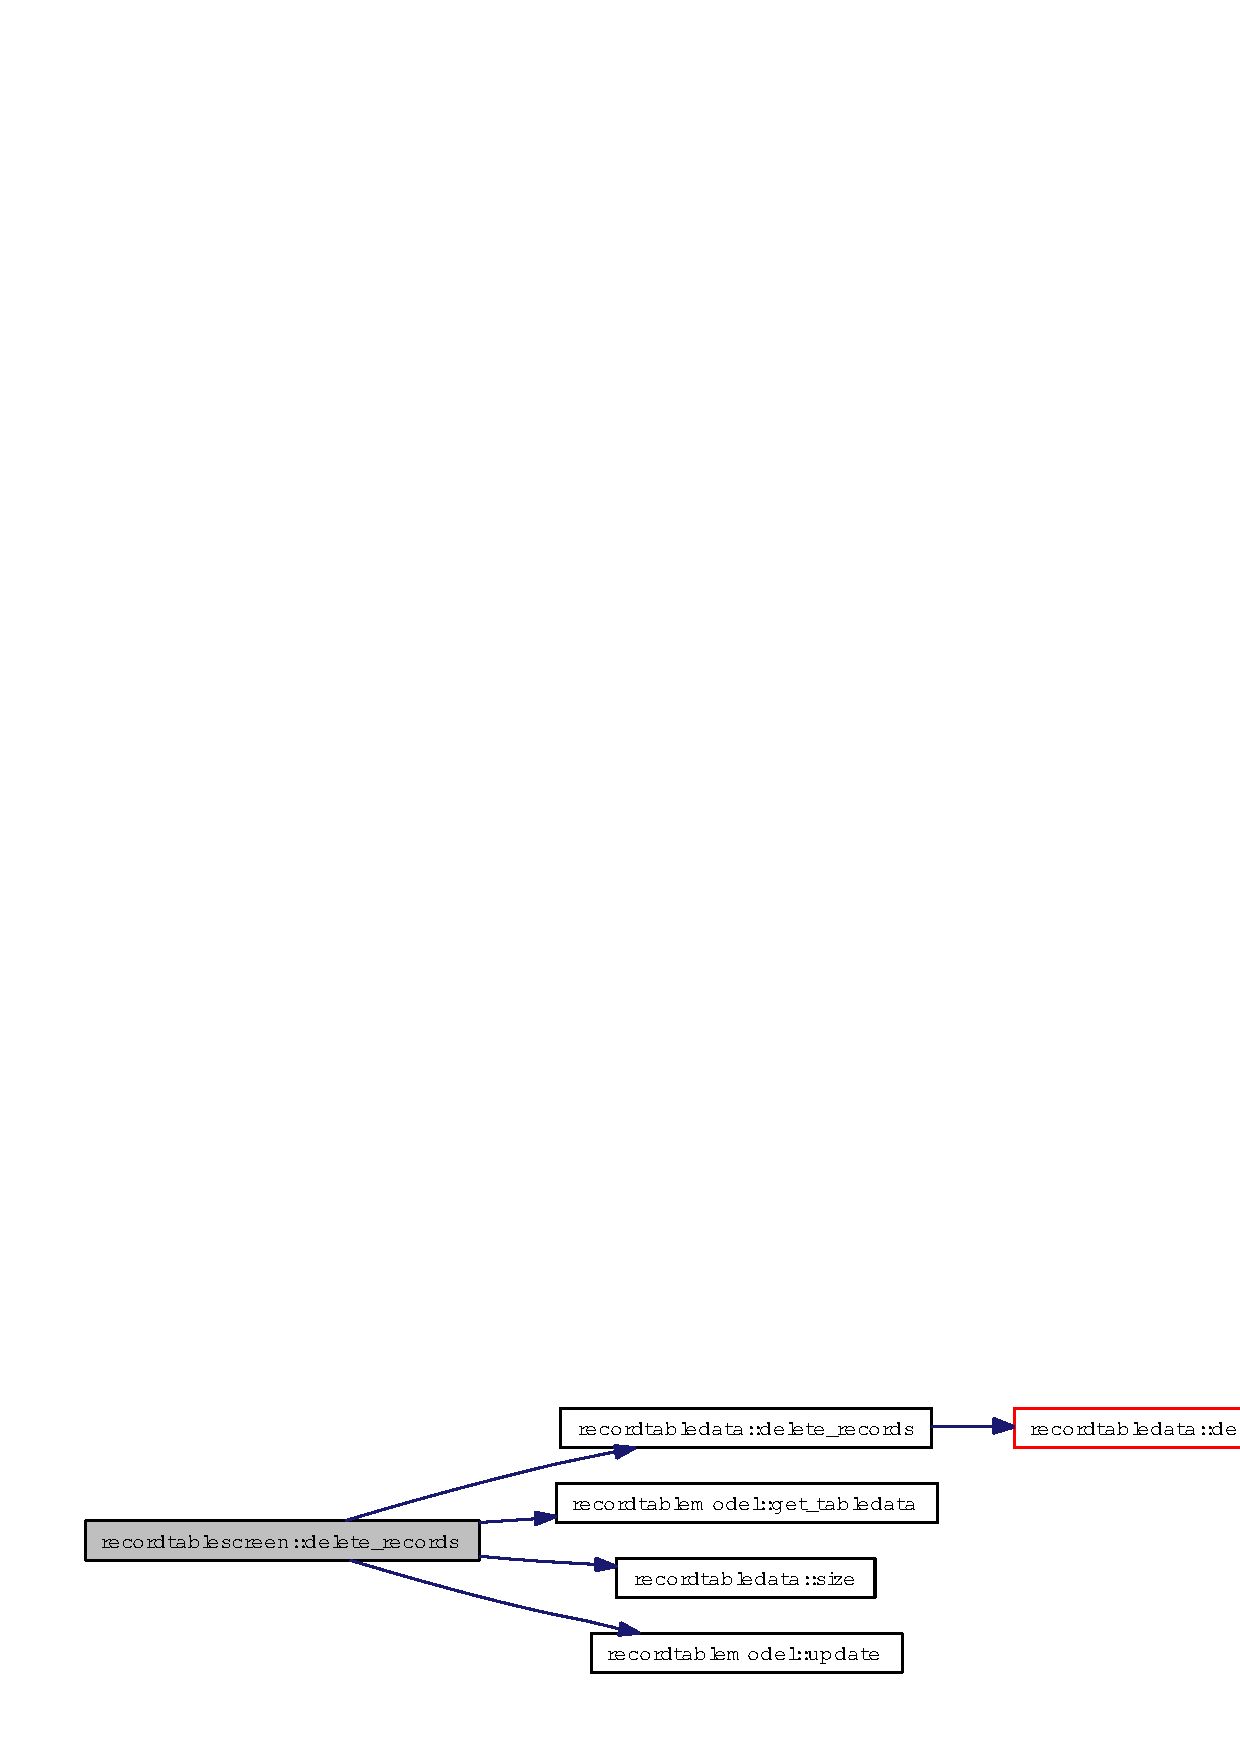
\includegraphics[width=332pt]{classrecordtablescreen_91d1bc4b540ad9af78437a59143e94a4_cgraph}
\end{center}
\end{figure}


\subsection{Member Data Documentation}
\index{recordtablescreen@{recordtablescreen}!tools_line@{tools\_\-line}}
\index{tools_line@{tools\_\-line}!recordtablescreen@{recordtablescreen}}
\subsubsection{\setlength{\rightskip}{0pt plus 5cm}QTool\-Bar$\ast$ {\bf recordtablescreen::tools\_\-line}\hspace{0.3cm}{\tt  [private]}}\label{classrecordtablescreen_4d12482b6d9a926f84b8095c1ca37683}




Definition at line 75 of file recordtablescreen.h.

Referenced by assembly(), and setup\_\-ui().\index{recordtablescreen@{recordtablescreen}!find_line@{find\_\-line}}
\index{find_line@{find\_\-line}!recordtablescreen@{recordtablescreen}}
\subsubsection{\setlength{\rightskip}{0pt plus 5cm}QTool\-Bar$\ast$ {\bf recordtablescreen::find\_\-line}\hspace{0.3cm}{\tt  [private]}}\label{classrecordtablescreen_79b4c677242dc0bbbf118bc7674c9d39}




Definition at line 76 of file recordtablescreen.h.

Referenced by assembly(), and setup\_\-ui().\index{recordtablescreen@{recordtablescreen}!recordview@{recordview}}
\index{recordview@{recordview}!recordtablescreen@{recordtablescreen}}
\subsubsection{\setlength{\rightskip}{0pt plus 5cm}QList\-View$\ast$ {\bf recordtablescreen::recordview}\hspace{0.3cm}{\tt  [private]}}\label{classrecordtablescreen_f155dacd499c3f6da2816da222683e87}




Definition at line 78 of file recordtablescreen.h.

Referenced by add\_\-new(), assembly(), copy(), delete\_\-records(), edit\_\-field\_\-context(), get\_\-first\_\-selection\_\-pos(), is\_\-selected\_\-set\_\-to\_\-bottom(), on\_\-custom\-Context\-Menu\-Requested(), recordtablescreen(), set\_\-selection\_\-to\_\-pos(), set\_\-tabledata(), setup\_\-signals(), setup\_\-ui(), and tools\_\-update().\index{recordtablescreen@{recordtablescreen}!recordmodel@{recordmodel}}
\index{recordmodel@{recordmodel}!recordtablescreen@{recordtablescreen}}
\subsubsection{\setlength{\rightskip}{0pt plus 5cm}{\bf recordtablemodel}$\ast$ {\bf recordtablescreen::recordmodel}\hspace{0.3cm}{\tt  [private]}}\label{classrecordtablescreen_1806a1e7cad7c5037c19ec88f3859f95}




Definition at line 79 of file recordtablescreen.h.

Referenced by add\_\-new(), copy(), delete\_\-records(), edit\_\-field(), edit\_\-field\_\-context(), movedn(), moveup(), recordtablescreen(), select(), set\_\-selection\_\-to\_\-pos(), and set\_\-tabledata().\index{recordtablescreen@{recordtablescreen}!recordtable_tools_layout@{recordtable\_\-tools\_\-layout}}
\index{recordtable_tools_layout@{recordtable\_\-tools\_\-layout}!recordtablescreen@{recordtablescreen}}
\subsubsection{\setlength{\rightskip}{0pt plus 5cm}QHBox\-Layout$\ast$ {\bf recordtablescreen::recordtable\_\-tools\_\-layout}\hspace{0.3cm}{\tt  [private]}}\label{classrecordtablescreen_7f35fe695ed9bf611d5c75a33e61693f}




Definition at line 81 of file recordtablescreen.h.

Referenced by assembly().\index{recordtablescreen@{recordtablescreen}!recordtablescreen_layout@{recordtablescreen\_\-layout}}
\index{recordtablescreen_layout@{recordtablescreen\_\-layout}!recordtablescreen@{recordtablescreen}}
\subsubsection{\setlength{\rightskip}{0pt plus 5cm}QVBox\-Layout$\ast$ {\bf recordtablescreen::recordtablescreen\_\-layout}\hspace{0.3cm}{\tt  [private]}}\label{classrecordtablescreen_7b65632d6fef4bd862e49ab1ec44846d}




Definition at line 82 of file recordtablescreen.h.

Referenced by assembly().\index{recordtablescreen@{recordtablescreen}!action_add_new_toend@{action\_\-add\_\-new\_\-toend}}
\index{action_add_new_toend@{action\_\-add\_\-new\_\-toend}!recordtablescreen@{recordtablescreen}}
\subsubsection{\setlength{\rightskip}{0pt plus 5cm}QAction$\ast$ {\bf recordtablescreen::action\_\-add\_\-new\_\-toend}\hspace{0.3cm}{\tt  [private]}}\label{classrecordtablescreen_755c98554622673eb9f70c0dff10074b}




Definition at line 84 of file recordtablescreen.h.

Referenced by disable\_\-all\_\-actions(), on\_\-custom\-Context\-Menu\-Requested(), setup\_\-actions(), setup\_\-ui(), and tools\_\-update().\index{recordtablescreen@{recordtablescreen}!action_add_new_before@{action\_\-add\_\-new\_\-before}}
\index{action_add_new_before@{action\_\-add\_\-new\_\-before}!recordtablescreen@{recordtablescreen}}
\subsubsection{\setlength{\rightskip}{0pt plus 5cm}QAction$\ast$ {\bf recordtablescreen::action\_\-add\_\-new\_\-before}\hspace{0.3cm}{\tt  [private]}}\label{classrecordtablescreen_6199377c78472f1c21b8ff6069f72c61}




Definition at line 85 of file recordtablescreen.h.

Referenced by disable\_\-all\_\-actions(), on\_\-custom\-Context\-Menu\-Requested(), setup\_\-actions(), and tools\_\-update().\index{recordtablescreen@{recordtablescreen}!action_add_new_after@{action\_\-add\_\-new\_\-after}}
\index{action_add_new_after@{action\_\-add\_\-new\_\-after}!recordtablescreen@{recordtablescreen}}
\subsubsection{\setlength{\rightskip}{0pt plus 5cm}QAction$\ast$ {\bf recordtablescreen::action\_\-add\_\-new\_\-after}\hspace{0.3cm}{\tt  [private]}}\label{classrecordtablescreen_350b6410856141258b1d324686e26b09}




Definition at line 86 of file recordtablescreen.h.

Referenced by disable\_\-all\_\-actions(), on\_\-custom\-Context\-Menu\-Requested(), setup\_\-actions(), and tools\_\-update().\index{recordtablescreen@{recordtablescreen}!action_edit_field@{action\_\-edit\_\-field}}
\index{action_edit_field@{action\_\-edit\_\-field}!recordtablescreen@{recordtablescreen}}
\subsubsection{\setlength{\rightskip}{0pt plus 5cm}QAction$\ast$ {\bf recordtablescreen::action\_\-edit\_\-field}\hspace{0.3cm}{\tt  [private]}}\label{classrecordtablescreen_3cbd66091b8a77cfa75ca9b61edc9f6f}




Definition at line 87 of file recordtablescreen.h.

Referenced by disable\_\-all\_\-actions(), on\_\-custom\-Context\-Menu\-Requested(), setup\_\-actions(), setup\_\-ui(), and tools\_\-update().\index{recordtablescreen@{recordtablescreen}!action_delete@{action\_\-delete}}
\index{action_delete@{action\_\-delete}!recordtablescreen@{recordtablescreen}}
\subsubsection{\setlength{\rightskip}{0pt plus 5cm}QAction$\ast$ {\bf recordtablescreen::action\_\-delete}\hspace{0.3cm}{\tt  [private]}}\label{classrecordtablescreen_fd4cb6265dd10d559f8d0244043dae42}




Definition at line 88 of file recordtablescreen.h.

Referenced by disable\_\-all\_\-actions(), on\_\-custom\-Context\-Menu\-Requested(), setup\_\-actions(), setup\_\-ui(), and tools\_\-update().\index{recordtablescreen@{recordtablescreen}!action_cut@{action\_\-cut}}
\index{action_cut@{action\_\-cut}!recordtablescreen@{recordtablescreen}}
\subsubsection{\setlength{\rightskip}{0pt plus 5cm}QAction$\ast$ {\bf recordtablescreen::action\_\-cut}\hspace{0.3cm}{\tt  [private]}}\label{classrecordtablescreen_7c31f0fce3ad60ad8117b6954f9bd875}




Definition at line 89 of file recordtablescreen.h.

Referenced by disable\_\-all\_\-actions(), on\_\-custom\-Context\-Menu\-Requested(), setup\_\-actions(), setup\_\-ui(), and tools\_\-update().\index{recordtablescreen@{recordtablescreen}!action_copy@{action\_\-copy}}
\index{action_copy@{action\_\-copy}!recordtablescreen@{recordtablescreen}}
\subsubsection{\setlength{\rightskip}{0pt plus 5cm}QAction$\ast$ {\bf recordtablescreen::action\_\-copy}\hspace{0.3cm}{\tt  [private]}}\label{classrecordtablescreen_7490f795a1262cf53d1f1e6455de0100}




Definition at line 90 of file recordtablescreen.h.

Referenced by disable\_\-all\_\-actions(), on\_\-custom\-Context\-Menu\-Requested(), setup\_\-actions(), setup\_\-ui(), and tools\_\-update().\index{recordtablescreen@{recordtablescreen}!action_paste@{action\_\-paste}}
\index{action_paste@{action\_\-paste}!recordtablescreen@{recordtablescreen}}
\subsubsection{\setlength{\rightskip}{0pt plus 5cm}QAction$\ast$ {\bf recordtablescreen::action\_\-paste}\hspace{0.3cm}{\tt  [private]}}\label{classrecordtablescreen_4a5328fc69bfc95fd33635bdd190da4a}




Definition at line 91 of file recordtablescreen.h.

Referenced by disable\_\-all\_\-actions(), on\_\-custom\-Context\-Menu\-Requested(), setup\_\-actions(), setup\_\-ui(), and tools\_\-update().\index{recordtablescreen@{recordtablescreen}!action_moveup@{action\_\-moveup}}
\index{action_moveup@{action\_\-moveup}!recordtablescreen@{recordtablescreen}}
\subsubsection{\setlength{\rightskip}{0pt plus 5cm}QAction$\ast$ {\bf recordtablescreen::action\_\-moveup}\hspace{0.3cm}{\tt  [private]}}\label{classrecordtablescreen_30cf00f9d33ba2dba680f9674abe5671}




Definition at line 92 of file recordtablescreen.h.

Referenced by disable\_\-all\_\-actions(), setup\_\-actions(), setup\_\-ui(), and tools\_\-update().\index{recordtablescreen@{recordtablescreen}!action_movedn@{action\_\-movedn}}
\index{action_movedn@{action\_\-movedn}!recordtablescreen@{recordtablescreen}}
\subsubsection{\setlength{\rightskip}{0pt plus 5cm}QAction$\ast$ {\bf recordtablescreen::action\_\-movedn}\hspace{0.3cm}{\tt  [private]}}\label{classrecordtablescreen_ccdcdeffdc381b2bdf2d8f550816d4ac}




Definition at line 93 of file recordtablescreen.h.

Referenced by disable\_\-all\_\-actions(), setup\_\-actions(), setup\_\-ui(), and tools\_\-update().\index{recordtablescreen@{recordtablescreen}!action_findinbase@{action\_\-findinbase}}
\index{action_findinbase@{action\_\-findinbase}!recordtablescreen@{recordtablescreen}}
\subsubsection{\setlength{\rightskip}{0pt plus 5cm}QAction$\ast$ {\bf recordtablescreen::action\_\-findinbase}\hspace{0.3cm}{\tt  [private]}}\label{classrecordtablescreen_5a75aaa4075022b193223603475aaef0}




Definition at line 94 of file recordtablescreen.h.

Referenced by setup\_\-actions(), and setup\_\-ui().\index{recordtablescreen@{recordtablescreen}!recordview_currentdir@{recordview\_\-currentdir}}
\index{recordview_currentdir@{recordview\_\-currentdir}!recordtablescreen@{recordtablescreen}}
\subsubsection{\setlength{\rightskip}{0pt plus 5cm}QString {\bf recordtablescreen::recordview\_\-currentdir}\hspace{0.3cm}{\tt  [private]}}\label{classrecordtablescreen_b7e9dbe44d4e786ac7aa1572990057d9}




Definition at line 101 of file recordtablescreen.h.

Referenced by get\_\-currentdir(), get\_\-fullfilename\_\-of\_\-currentitem(), recordtablescreen(), select(), and set\_\-tabledata().\index{recordtablescreen@{recordtablescreen}!recordview_currentfile@{recordview\_\-currentfile}}
\index{recordview_currentfile@{recordview\_\-currentfile}!recordtablescreen@{recordtablescreen}}
\subsubsection{\setlength{\rightskip}{0pt plus 5cm}QString {\bf recordtablescreen::recordview\_\-currentfile}\hspace{0.3cm}{\tt  [private]}}\label{classrecordtablescreen_c95f81253a5ba51b15a9c2fdea58b436}




Definition at line 102 of file recordtablescreen.h.

Referenced by get\_\-currentfile(), get\_\-fullfilename\_\-of\_\-currentitem(), recordtablescreen(), select(), and set\_\-tabledata().

The documentation for this class was generated from the following files:\begin{CompactItemize}
\item 
{\bf recordtablescreen.h}\item 
{\bf recordtablescreen.cpp}\end{CompactItemize}
